\documentclass[MTech]{iitddiss}
% \settopmatter{printacmref=false}

\input{macros}
\usepackage{t1enc}

\usepackage{graphicx}
\usepackage{hyperref} % hyperlinks for references.
\usepackage{amsmath} % easier math formulae, align, subequations \ldots
\usepackage[english]{babel}
\usepackage[utf8]{inputenc}
\usepackage{natbib}
\usepackage{fancyhdr}
 \linespread{1.2}

\pagestyle{fancy}
\renewcommand{\sectionmark}[1]{\markright{\thesection\ #1}}

\fancyhf{}

\rhead{\fancyplain{}{\thepage}} % predefined ()
\lhead{\fancyplain{}{\rightmark}} % 1. sectionname, 1.1 subsection name etc
\cfoot{\textcopyright \text{ } \the\year, \emph{Indian Institute of Technology Delhi}}
\renewcommand{\footrulewidth}{0.4pt}
\begin{document}


%%%%%%%%%%%%%%%%%%%%%%%%%%%%%%%%%%%%%%%%%%%%%%%%%%%%%%%%%%%%%%%%%%%%%%
% Title page

\title{An Approximate Algorithm for Mining Top-$k$ Correlated Subgraphs in a Large Graph}

\author{Arneish Prateek}
\advisor{Prof. Sayan Ranu}
\entrynumber{2014CH10786}
\date{June 2019}
\department{Computer Science and Engineering}

%\nocite{*}
\maketitle


% \pagenumbering{arabic}

% \copyrightyear{2020}
% \acmYear{2020}
% \setcopyright{acmcopyright}
% \acmConference[SIGMOD '20]{ACM SIGMOD '20: ACM International Conference on Management of Data}{June 14--19, 2020}{Portland, Oregon, USA}
% \acmPrice{15.00}
% \acmDOI{10.1145/1122445.1122456}
% \acmISBN{978-1-4503-9999-9/18/06}

% \begin{document}

% \title{}

% \author{}
% \advisor{Sayan Ranu}
% \department{Computer Science and Engineering}

%\author{Arijit Khan} \affiliation{\institution{Nanyang Technological
%University}
%}
%\email{arijit.khan@ntu.edu.sg}
%
%\author{Arneish Prateek} \affiliation{\institution{Indian Institute of
%Technology Delhi, India}
%}
%\email{ch1140786@iitd.ac.in}
%
%\author{Sayan Ranu} \affiliation{\institution{Indian Institute of Technology
%Delhi, India}
%}
%\email{sayanranu@iitd.ac.in}
%
%\author{Akshit Goyal} \affiliation{\institution{Indian Institute of Technology
%Delhi, India}
%}
%\email{cs5140278@iitd.ac.in}

% \maketitle

%%%%%%%%%%%%%%%%%%%%%%%%%%%%%%%%%%%%%%%%%%%%%%%%%%%%%%%%%%%%%%%%%%%%%%
% Certificate
\certificate

\vspace*{0.5in}

\noindent This is to certify that the thesis titled {\bf\ An Approximate
Algorithm for Mining Top-$k$ Correlated Subgraphs in a Large Graph} submitted
by {\bf Arneish Prateek}, to Indian Institute of Technology, Delhi, for
the award of the degree of {\bf Master of Technology}, is a bonafide
record of the research work done by him under our supervision.  The
contents of this thesis, in full or in parts, have not been submitted
to any other Institute or University for the award of any degree or
diploma.

\vspace*{1.5in}

\begin{singlespacing}
\hspace*{-0.25in}
\parbox{2.5in}{
\noindent {\bf Prof.~1} \\
\noindent Professor Sayan Ranu\\
\noindent Dept of CSE\\
\noindent IIT-Delhi, 110016 \\
}
\hspace*{1.0in}
\end{singlespacing}
\vspace*{0.25in}
\noindent \hfill Place: New Delhi\\
\noindent \hfill Date: June 25, 2019\\

%%%%%%%%%%%%%%%%%%%%%%%%%%%%%%%%%%%%%%%%%%%%%%%%%%%%%%%%%%%%%%%%%%%%%%
% Acknowledgements

\acknowledgements

This thesis is the outcome of a joint collaborative effort with \textbf{Akshit Goyal}
(Master's Candidate, IIT Delhi). The author of this thesis has attempted to
demarcate the contributions of the collaborator and himself to the best of his
abilities. For a complete guide to this project, this thesis must be read in
conjunction with the thesis titled \textbf{An Exact Algorithm for Mining Top-$k$
Correlated Subgraphs in a Large Graph} by \textbf{Akshit Goyal}. Appendix I contains
the complementary sections from this other thesis. The following chapters are
common to both theses:

\textbf{Chapter 1}

\textbf{Chapter 2}

\textbf{Chapter 3}: Sections 3.1,3.2,3.3,3.4

\textbf{Chapter 4}: Section 4.1



\begin{abstract}
	Mining of correlated patterns, that represent an important class of
	regularities, has become increasingly important in data management and
	analytics. Surprisingly, the problem of correlated subgraphs mining from a
	single, large graph has received little attention. We investigate a novel and
	critical graph mining problem, called {\em correlated subgraphs mining} ({\sf{CSM}}), 
	which is defined as a pair of subgraph patterns that frequently co-occur in proximity
	within a single graph.
	
	Correlated subgraphs are different from frequent subgraphs due to the
	flexibility in which the constituent subgraph instances are connected, thus the
	existing frequent subgraphs mining algorithms cannot be directly applied.
	Furthermore, correlation computation between two subgraph patterns require
	enumerating and finding distances between every pair of subgraph instances of
	both these patterns --- which is memory intensive and computationally
	demanding.
	
	To this end, we design two novel, holistic, best-first exploration algorithms: {\sf{CSM-E}}
	(an exact method) and {\sf{CSM-A}} (a more efficient, approximate method with near-optimal
	quality). To further improve their efficiency, we propose a top-$k$ pruning strategy, 
	while to reduce memory footprints, we develop a compressed data structure, 
	$\mathcal{R}$eplica, that stores all instances of a subgraph pattern on demand. 
	Our empirical results show that the proposed algorithms not only find interesting correlations, 
	but also achieve good scalability over large networks.
	\end{abstract}

%%%%%%%%%%%%%%%%%%%%%%%%%%%%%%%%%%%%%%%%%%%%%%%%%%%%%%%%%%%%%%%%%
% Table of contents etc.

\begin{singlespace}
\tableofcontents
\thispagestyle{empty}

% \listoftables
% \addcontentsline{toc}{chapter}{LIST OF TABLES}
% \listoffigures
% \addcontentsline{toc}{chapter}{LIST OF FIGURES}
\end{singlespace}





%%%%%%%%%%%%%%%%%%%%%%%%%%%%%%%%%%%%%%%%%%%%%%%%%%%%%%%%%%%%%%%%%%%%%%
% Abbreviations
% \abbreviations

% \noindent
% \begin{tabbing}
% xxxxxxxxxxx \= xxxxxxxxxxxxxxxxxxxxxxxxxxxxxxxxxxxxxxxxxxxxxxxx \kill
% \textbf{IITD}   \> Indian Institute of Technology, Delhi \\
% \textbf{RTFM} \> Read the Fine Manual \\
% \end{tabbing}

% \pagebreak

%%%%%%%%%%%%%%%%%%%%%%%%%%%%%%%%%%%%%%%%%%%%%%%%%%%%%%%%%%%%%%%%%%%%%%
% Notation

% \chapter*{\centerline{NOTATION}}
% \addcontentsline{toc}{chapter}{NOTATION}

% \begin{singlespace}
% \begin{tabbing}
% xxxxxxxxxxx \= xxxxxxxxxxxxxxxxxxxxxxxxxxxxxxxxxxxxxxxxxxxxxxxx \kill
% \textbf{$r$}  \> Radius, $m$ \\
% \textbf{$\alpha$}  \> Angle of thesis in degrees \\
% \textbf{$\beta$}   \> Flight path in degrees \\
% \end{tabbing}
% \end{singlespace}

% \pagebreak
% \clearpage

% The main text will follow from this point so set the page numbering
% to arabic from here on.
\pagenumbering{arabic}

\vspace{-4mm}




\section{Introduction}
\label{sec:intro}

Graphs are a ubiquitous model to represent objects and their complex relations,
including protein interaction networks and genomic graphs in biology \cite{RHS13},
chemical compounds \cite{WMFP05}, call graphs in program flow analysis \cite{control},
social networks \cite{Kempe}, and government and medical records \cite{SH12}.
Efficient mining of hidden patterns play an important role in developing data-driven
methodologies for analyzing graphs
resulting from such datasets.
Research on graph mining has emerged as one of the hottest topics in recent years due to its wide applications in a variety of fields including
drug discovery \cite{KK01,NK05,YH02}, molecular activity prediction \cite{JinYW10,TCG09},
predicting disease susceptibility from gene expression data \cite{RHS13,DI11}, clustering and classification of graphs \cite{DKWK05,YCHY08}, and anomaly detection \cite{ATK15}.
Several variants of graph pattern mining have been proposed,
such as frequent subgraphs \cite{YH02,EASK14}, approximate subgraphs \cite{KYW10}, discriminant and statistically significant subgraphs \cite{TCG09,RS09,YCHY08}, representative subgraphs \cite{CHSBZ08,ZYL09}, etc.
%--- their scalable algorithms
%were implemented; besides, they were extensively surveyed and compared, e.g., in \cite{HCXY07,WMFP05,AW10,KR17}.
%
\begin{figure}[t!]
\vspace{-2mm}
\centering
\includegraphics[width=2.2in]{images/taxol.pdf}
\caption{Correlation between {\sf CCCH} and {\sf O} in {\sf Taxol}, an anti-cancer drug. {\sf CCCH} and {\sf O}
occur closely for several times, but they are connected in different ways.}
\label{fig:taxol}
\vspace{-0.10in}
\end{figure}
%


In spite of tremendous progress being made in the area of graph pattern mining, surprisingly the problem of exploring correlations between subgraphs
in a single, large graph has not been investigated in the past. In particular, we define a pair of subgraphs as correlated if
they co-occur frequently in proximity within a single graph. Correlated subgraphs are different from frequent subgraphs due to
the flexibility in which the constituent subgraphs can be connected within different instances of a correlated pattern. To elaborate, in Figure~\ref{fig:taxol},
we highlight three regions inside the structure of the chemical compound {\sf Taxol}, an anti-cancer drug, where {\sf CCCH} and {\sf O} occur closely,
albeit they are connected in different ways in all three instances. For simplicity, we do not consider the edge types (i.e., single- vs. double-bond)
in this example. This figure illustrates that while {\sf CCCH} and {\sf O} form a correlated subgraph pair, the individual instances, e.g., {\sf HCC(-O)C}
may not be frequent; and hence, existing frequent subgraphs mining techniques would not discover such corrected patterns.

\vspace{-0.05in}
\subsection{Applications}
The problem of detecting correlated subgraphs from a single, large graph arises in many real-world scenarios, including biological,
social, chemical, and ecological networks. We discuss two concrete examples below.

\begin{figure}
 \vspace{-0.20in}
 \centering
	\begin{subfigure}[t]{0.21\textwidth}
		\includegraphics[scale=0.24]{img2/mico/mico_gvf3.pdf}
		\caption{\scriptsize $Mico$ dataset (small)}
		\label{fig:intro_micogvf3}
    \end{subfigure}%
    \hspace*{\fill}
	\begin{subfigure}[t]{0.23\textwidth}
		\includegraphics[scale=0.24]{img2/citationdblp/citationdblp_gvf3.pdf}
		\caption{\scriptsize $DBLP\ Citation$ dataset (large)}
		\label{fig:intro_citationdblpgvf3}
	\end{subfigure}%
	\caption{Our performance against GraMi+VF3 baseline}
	\label{fig:motivation}
	\vspace{-0.1in}
\end{figure}

\spara{$\bullet$ Co-operative functions in biological networks.} In genome graph of an individual, a node represents a gene,
and each edge denotes the interaction between two genes. In practice, there are some combinations of dominant genes that
occur frequently, and they are more likely to express critical phenotypes of the individual.
Past studies have shown that some pairs of dominant gene combinations co-occur with each other in each individual,
and such co-occurring patterns reflect the joint functionality that are needed for co-operative biological functions such as chemical bonds
and binding sites \cite{LFSW14}. Based on pairs of correlated genes, we can predict co-operative biological functions of an
individual. Besides, the absence of such correlations indicates anomalies and diseases.
Analogously, in a protein interaction network, correlated frequent subgraphs represent recurring functional units,
identification of which could assist in predicting new protein functionalities.

%\vspace{-0.05in}
\spara{$\bullet$ Co-occurrence patterns in ecological networks.}
In ecology, co-occurrence patterns are used to explore interactions between organisms
and environmental effects on co-existence within biological communities \cite{WHH14}.
Exploration of inter-taxa relationships can help identify potential biotic interactions, habitat affinities, and shared physoilogies,
that could guide more focused studies and experiments. For example, Barberan et al. \cite{BBCF12} analyzed
over $160\,000$ bacterial and archaeal $16S$ rRNA gene sequences from $151$ soil samples, collected
from a wide variety of ecosystem types, in order to demonstrate the utility of network
analyses and for evaluating whether soil microorganisms tend to co-occur more
than expected by chance, and how these
ecological categories shape network structure of inter-taxa and extra-taxa relationships.
These tasks can be achieved by mining correlated subgraphs in a single large graph
representing the soil microbial community.

\vspace{-0.05in}
\subsection{Technical Challenges and Baselines}
\label{sec:baseline}
%The problem that we study is a non-trivial one.
%
%\squishlist
\textbf{Frequent subgraphs mining. } Detecting correlated subgraphs is more difficult
than the frequent subgraphs mining problem \cite{WMFP05}, which already has an exponential search space, that is, a graph with $m$ edges
can have $2^m$ subgraphs. For correlated subgraphs mining, the search space is doubly-exponential, because
one needs to compute the correlation between every pair of subgraph instances.
 Additionally, unlike frequent subgraphs mining,
correlated subgraphs mining is neither downward-closure, nor upward-closure (we shall demonstrate this formally
in \S~\ref{sec:problem}), thereby making it difficult to directly apply apriori-based pruning techniques.

 Last, but not least, only finding the frequent subgraphs is not sufficient for our problem. Since we call subgraph $A$ to be correlated to $B$ if their \emph{instances} are frequently located close to each other, we need to enumerate \emph{all} instances of those frequent subgraphs for computing the correlation
between pairs. This makes our problem more challenging both from computation and memory perspective. To establish this point empirically, we perform frequent subgraphs mining using GraMi~\cite{EASK14}, and for each frequent subgraph, we enumerate all of its instances using the state-of-the-art VF3 algorithm~\cite{CarlettiFSV18} and finally compute the correlated pairs. Fig.~\ref{fig:motivation} presents the result on two datasets; the dataset description is provided in Table~\ref{ref:datasets}. We observe that the frequent subgraphs mining based approach takes more than $15$ days in the DBLP-Citation network dataset. On the other hand, the proposed approach, CSM, is up to $5$ orders of magnitude faster. Real networks contain millions of nodes and it is desirable to obtain results within minutes. In this paper, we achieve this task with a single-step correlated subgraphs mining algorithm. %As visible in Fig.~\ref{fig:motivation}, the proposed approach, denoted as CSM, is XXX orders of magnitude faster.


\textbf{Correlated subgraphs mining in graph databases. } The closest work to ours in the space of correlated subgraphs mining is by Ye et al.\cite{KCY09}. However, there are three fundamental differences. First, Ye et al. target the graph database scenario where there are multiple graphs and the frequency of a subgraph is defined as the number of database graphs containing the given subgraph. In our problem, we target the single large graph scenario where the frequency of a subgraph is the number instances within the single large graph. It is well known from the frequent subgraphs mining literature \cite{EASK14,KhanR17}, that the single-large-graph scenario imposes a more severe scalability challenge since subgraph enumeration is more expensive. Second, the definition of correlated patterns is different. More specifically, in \cite{KCY09}, two subgraphs $A$ and $B$ are correlated if the containment of $A$ within a data graph increases the likelihood of containing $B$ as well. In our problem, two subgraphs $A$ and $B$ are correlated if the instances of $A$ are frequently located in \emph{close proximity} to the instances of $B$. Third, we have the concept of proximity in our problem, which is absent in \cite{KCY09}. Owing to these fundamental differences in the formulation, the resulting algorithmic challenges are different as well.

%We next describe why state-of-the-art techniques cannot be trivially adapted to find correlated subgraphs
%in a single, large graph.
%
%\spara{$\bullet$ Difficulties with Frequent Subgraphs Enumeration.}
%One can apply state-of-the-art frequent subgraphs mining techniques over a single graph (e.g., {\sf GRAMI} \cite{EASK14})
%to first identify all frequent subgraphs, compute correlations between every pair, and then report the
%highly correlated ones. However, this approach has several limitations.
%{\bf (1)} Many existing frequent subgraphs mining algorithms including {\sf GRAMI}
%report only the frequent subgraphs, and not their instances in the large graph.
%Thus, we separately need to enumerate all their instances using a subgraph matching algorithm
%(e.g., {\sf VF2} \cite{CFSV04}, $\textsf{Turbo}_\textsf{ISO}$ \cite{HLL13}, $\textsf{Dual}_\textsf{ISO}$ \cite{SJKFMR14}),
%which is necessary for correlation computation, but is expensive over large graphs (Figure XX).
%{\bf (2)} We are often interested in finding only the top-$k$ correlated pairs. However, the aforementioned
%frequent subgraphs mining and enumeration approach will compute correlations across every frequent subgraphs,
%which is expensive and mostly redundant. This brings the following critical question: {\em Can we mine the (top-$k$) correlated
%subgraphs in one single step}, as opposed to the aforementioned two-step frequent subgraphs mining and enumeration approach?
%The answer to this question, as we shall demonstrate in \S~\ref{sec:algorithms}, is affirmative.
%
%\begin{figure}[t!]
%\vspace{-2mm}
%\centering
%\subfigure[] {
%\includegraphics[scale=0.17]{images/yeast1}
%\label{fig:yeast1}
%}
%\subfigure[]  {
%\includegraphics[scale=0.17]{images/yeast2}
%\label{fig:yeast2}
%}
%\subfigure[]  {
%\includegraphics[scale=0.17]{images/yeast3}
%\label{fig:yeast3}
%}
%\vspace{-2mm}
%\caption{\scriptsize Correlated subgraphs discovered in the {\em Yeast} protein dataset. Nodes are annotated with protein functions (node labels).}
%\label{fig:yeast}
%\vspace{-6mm}
%\end{figure}


%\spara{$\bullet$ Difficulties with Proximity Patterns.} Recently, various approximate-frequent-subgraphs mining techniques have been
%proposed, e.g., proximity patterns \cite{KYW10} that relax the rigid structure constraint of frequent subgraphs. In stead, they identify
%a group of node labels that co-occur frequently in the neighborhood. However, such proximity patterns are often unable to capture
%the semantics of our novel correlated subgraphs. As an example, in Figure~\ref{fig:yeast},
%we present three correlated patterns identified from
%the {\em Yeast} (Saccharomyces cerevisiae) protein dataset \cite{}, where protein functions are used as node labels. These
%correlated patterns indicate that {\em transferase} and {\em hydrolase} activities are associated with {\em ion} binding,
%which is due to the fact that {\em transferase} and {\em hydrolase} undergo motions upon ligand ({\em ion}) binding
%to achieve their functions \cite{KAOK08}. However, {\em transferase} and {\em hydrolase} catalyze different chemical
%reactions and express different dynamic responses upon ligand ({\em ion}) binding. It means that {\em hydrolase} and {\em transferase}
%activities are usually not connected with each other directly and they usually connect to {\em ion} binding \cite{KKO09}.
%This is indeed reflected in our discovered correlated patterns, because there is no direct edge between {\em hydrolase} and {\em transferase}.
%On the other hand, the proximity pattern mining algorithm \cite{KYW10} reports
%$\langle${\em hydrolase}, {\em transferase}, {\em ion binding}$\rangle$ as one
%proximity pattern, thus it is unable to capture the fact that {\em hydrolase} and {\em transferase}
%activities are not connected with each other directly.

\vspace{-0.1in}
\subsection{Contributions and Roadmap}
%In this paper, we design a single-step, best-first exploration algorithm to detect correlated subgraphs,
%coupled with efficient top-$k$ pruning and various optimization techniques.
The main contributions of this paper are as follows:
\squishlist
\item We formulate the problem of \emph{correlated subgraphs mining} in a single large graph, which is defined as a pair of subgraph patterns that frequently
co-occur in proximity within a single graph (\S~\ref{sec:preliminaries}).
\item The key differentiating factor in our problem compared to existing subgraph mining problems is that we not only need to identify the subgraph patterns, but also enumerate and store all of its instances. This requirement imposes a huge scalability challenge on both computation and storage. We tackle this issue by designing a novel data structure called \emph{$\mathcal{R}$eplica}, which stores all instances of a subgraph pattern on demand in compressed manner. %$\mathcal{R}$eplica not only brings down the computation cost, but also reduces the storage cost drastically. 
 Using $\mathcal{R}$eplica as the data storage platform, we design a single-step, best-first exploration algorithm to detect correlated subgraph pairs efficiently (\S 3). We further speed up the mining process by designing a near-optimal approximtion algorithm (\S 4).
\item We empirically demonstrate effectiveness and efficiency of our methods on seven real graphs, while also detailing concrete case studies. We establish that the proposed algorithm is up to $5$ orders of magnitude faster than baseline strategies and scalable in million-sized networks (\S \ref{sec:experiments}).
\squishend

\section{Preliminaries}
\label{sec:preliminaries}
%
\subsection{Background}
\label{sec:background}
%
A data graph $G = (V,E,L)$ has a set of nodes $V$, a set of edges
$E \subseteq V \times V$, and a label set $\mathbb{L}$ s.t.
every node $v \in V$ is associated with a label, i.e., $L(v) \in \mathbb{L}$.
For simplicity, we focus on bidirectional, node labeled, and unweighted
graphs. However, the proposed models and algorithms can also be applied to weighted
and edge labeled graphs, e.g., in our experiments (\S~\ref{sec:experiments}), we demonstrate results over
edge labeled graphs.

\spara{Subgraph Isomorphism.} Given a data graph $G=(V,E,L)$, a graph pattern
$Q=(V_Q,E_Q,L_Q)$, a subgraph isomorphism is an {\em injective function} $M: V_Q \rightarrow V$ s. t.
{\bf (1)} $\forall v\in V_Q, L_Q(v)= L(M(v))$, and {\bf (2)} $\forall(v_1,v_2) \in E_Q, (M(v_1),M(v_2))\in E$.
%
\begin{figure}[t!]
\centering
\vspace{-1\baselineskip}
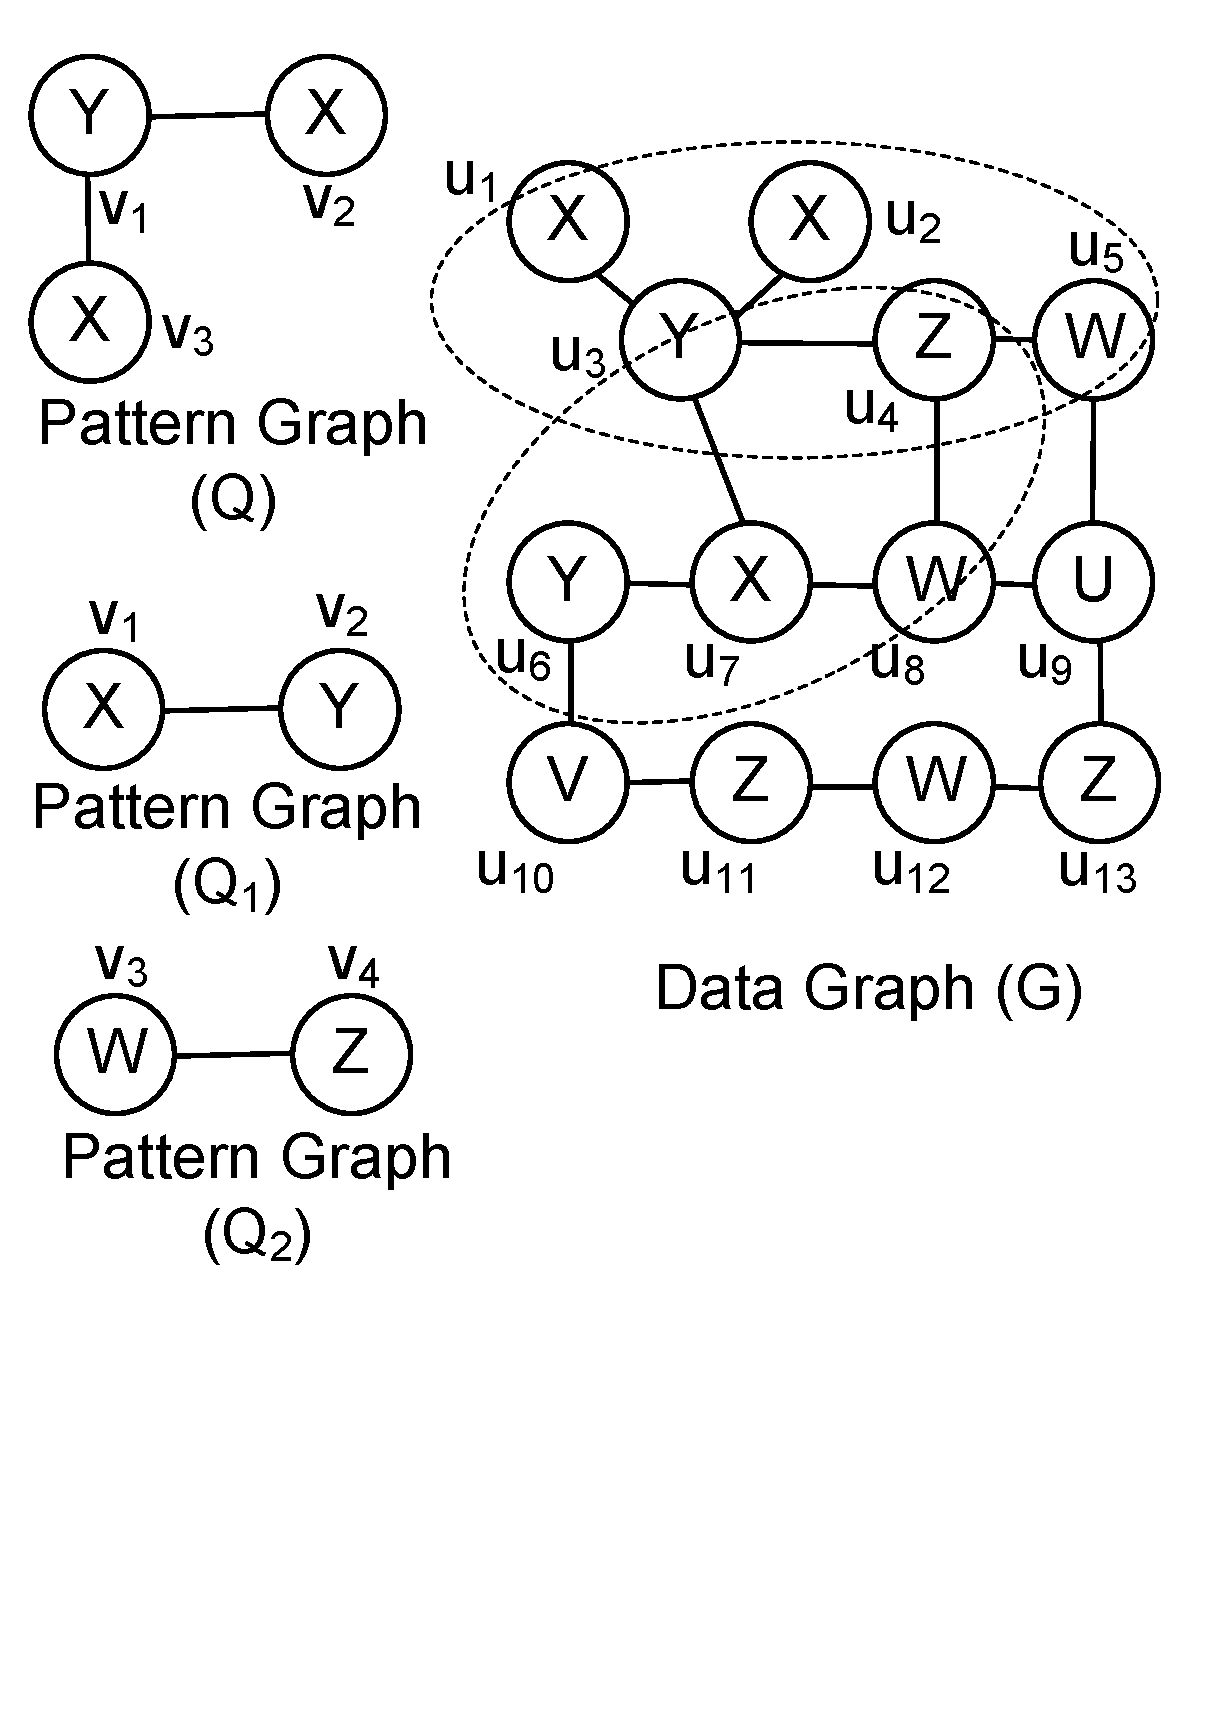
\includegraphics[scale=0.23]{images/correlation}
%\vspace{-1\baselineskip}
\caption{Subgraph isomorphism from $Q$ to $G$. Correlation between $Q_1$ and $Q_2$ in $G$.}
\label{fig:subgraph_isomorphism}
\vspace{-0.1\baselineskip}
\end{figure}

\spara{Support.}
To find frequent subgraphs\footnote{{\footnotesize We use `subgraph' and `subgraph pattern' interchangeably in the paper.}}
from a single, large graph, several definitions of subgraph support ($\sigma$)
have been proposed, e.g., maximum independent sets (MIS) \cite{KK04},
minimum image-based (MNI) \cite{BN08}, and harmful overlap (HO) \cite{FB07}.
We adopt MNI  \cite{BN08}
due to following reasons. {\bf (1)} MNI
can be efficiently computed from subgraph isomorphic instances;
whereas the computation of MIS and HO are \NP-complete \cite{KK04,FB07}.
{\bf (2)} MNI provides a superset of results of the two other metrics; thus
MIS or HO-based results can be identified via an expensive postprocessing step
\cite{EASK14}. {\bf (3)} MNI (as well as two other metrics) is {\em downward closure}:
The support of a supergraph $Q_1 \succeq Q$ is smaller (or equal) than that
of its subgraph $Q$, i.e., $\sigma(Q_1) \le \sigma(Q)$.

\spara{Minimum Image-based (MNI) Support \cite{BN08}.}
It is based on the number of unique nodes in $G$ that a node of the pattern $Q$
is mapped to. Formally,
%
\begin{align}
\displaystyle \sigma(Q) = \min_{v \in V_Q} |\{M(v) : M \,\text{is a subgraph isomorphic mapping}\}| \nonumber &
\end{align}
%
\begin{exple}
Figure~\ref{fig:subgraph_isomorphism} shows subgraph isomorphism. For a subgraph isomorphic
{\em mapping} $M$, the nodes $\{M(v):v\in V_Q\}$ and the corresponding edges $\{(M(v_1),M(v_2)):(v_1,v_2)\in E_Q\}$
form a subgraph isomorphic {\em instance} of $Q$ in $G$.
There can be many subgraph isomorphic mappings and instances, e.g.,
{\bf (1)} $M_1(v_1)= u_3$, $M_1(v_2)= u_2$, $M_1(v_3)= u_7$; {\bf (2)} $M_2(v_1) = u_3$, $M_2(v_2) = u_1$,
$M_2(v_3) = u_2$, etc. The MNI support of $Q$ is $1$, which is due to
node $v_1$: It is mapped to only one node in $G$, i.e., $u_3$ for all
mappings. The nodes in the set $\{M(v)\}$ for different mappings $M$ are called the {\em images} of $v$.
\end{exple}

\spara{Frequent Subgraphs.} Given the data graph $G$, a user-defined minimum support threshold $\Sigma$, and
a definition of support $\sigma$, the frequent subgraphs mining problem identifies all subgraphs $Q$ of $G$, such that
$\sigma(Q)\ge$ $\Sigma$.
%
\subsection{Problem Formulation}
\label{sec:problem}
%
Informally speaking, our objective is to identify those pairs of subgraph patterns $\langle Q_1, Q_2\rangle$ such that
they occur closely for a sufficiently large number of times in the data graph $G$. We formalize this notion of
correlation by incorporating the following constraints: {\bf (1)} The correlation between two subgraph patterns must be
symmetric, and {\bf (2)} it shall be consistent with the definition of MNI support.

For consistency with MNI, we group subgraph instances.
%
\begin{defn}[Instance Grouping]
\label{def:instance_grouping}
Given the data graph $G$, a graph pattern $Q$, and its instances in $G$ denoted as $\mathbb{I}=\{I_1,I_2,\ldots,I_s\}$,
let us define by $v^*$ the node in $Q$ which has the minimum number of images. We denote by
$\mathbb{M}(v^*)=\{M_1(v^*),M_2(v^*),\ldots,M_{\sigma(Q)}(v^*)\}$ the images of $v^*$. Notice that
$\sigma(Q)$ is the MNI support of $Q$, $\sigma(Q)\le s$, and $M_j(v^*)\in G$ is
a mapping of $v^*\in Q$, for all $1 \le j \le \sigma(Q)$. Next, we form a grouping
of instances, denoted as $\mathbb{I'}=\{I'_1,I'_2,\ldots,I'_{\sigma(Q)}\}$, where
$I'_j= \{I:M_j(v^*) \in I, I \in \mathbb{I}\}$. Intuitively,
$I'_j$ is the group of instances containing the image node $M_j(v^*)$.
\end{defn}
%
\begin{exple}
For data graph $G$ and graph pattern $Q_1$ in Figure~\ref{fig:subgraph_isomorphism},
the instances are
given by $\mathbb{I}=\{u_1u_3,u_2u_3,u_7u_3,u_7u_6\}$. However, its MNI support is two, since
node $v_2$ has only two corresponding images: $u_3$ and $u_6$. Thus, we group the instances
according to the presence of $u_3$ and $u_6$ as follows: $\mathbb{I'}=\{u_1u_2u_7u_3,u_7u_6\}$.
\end{exple}
%
%\begin{figure}[t!]
%\centering
%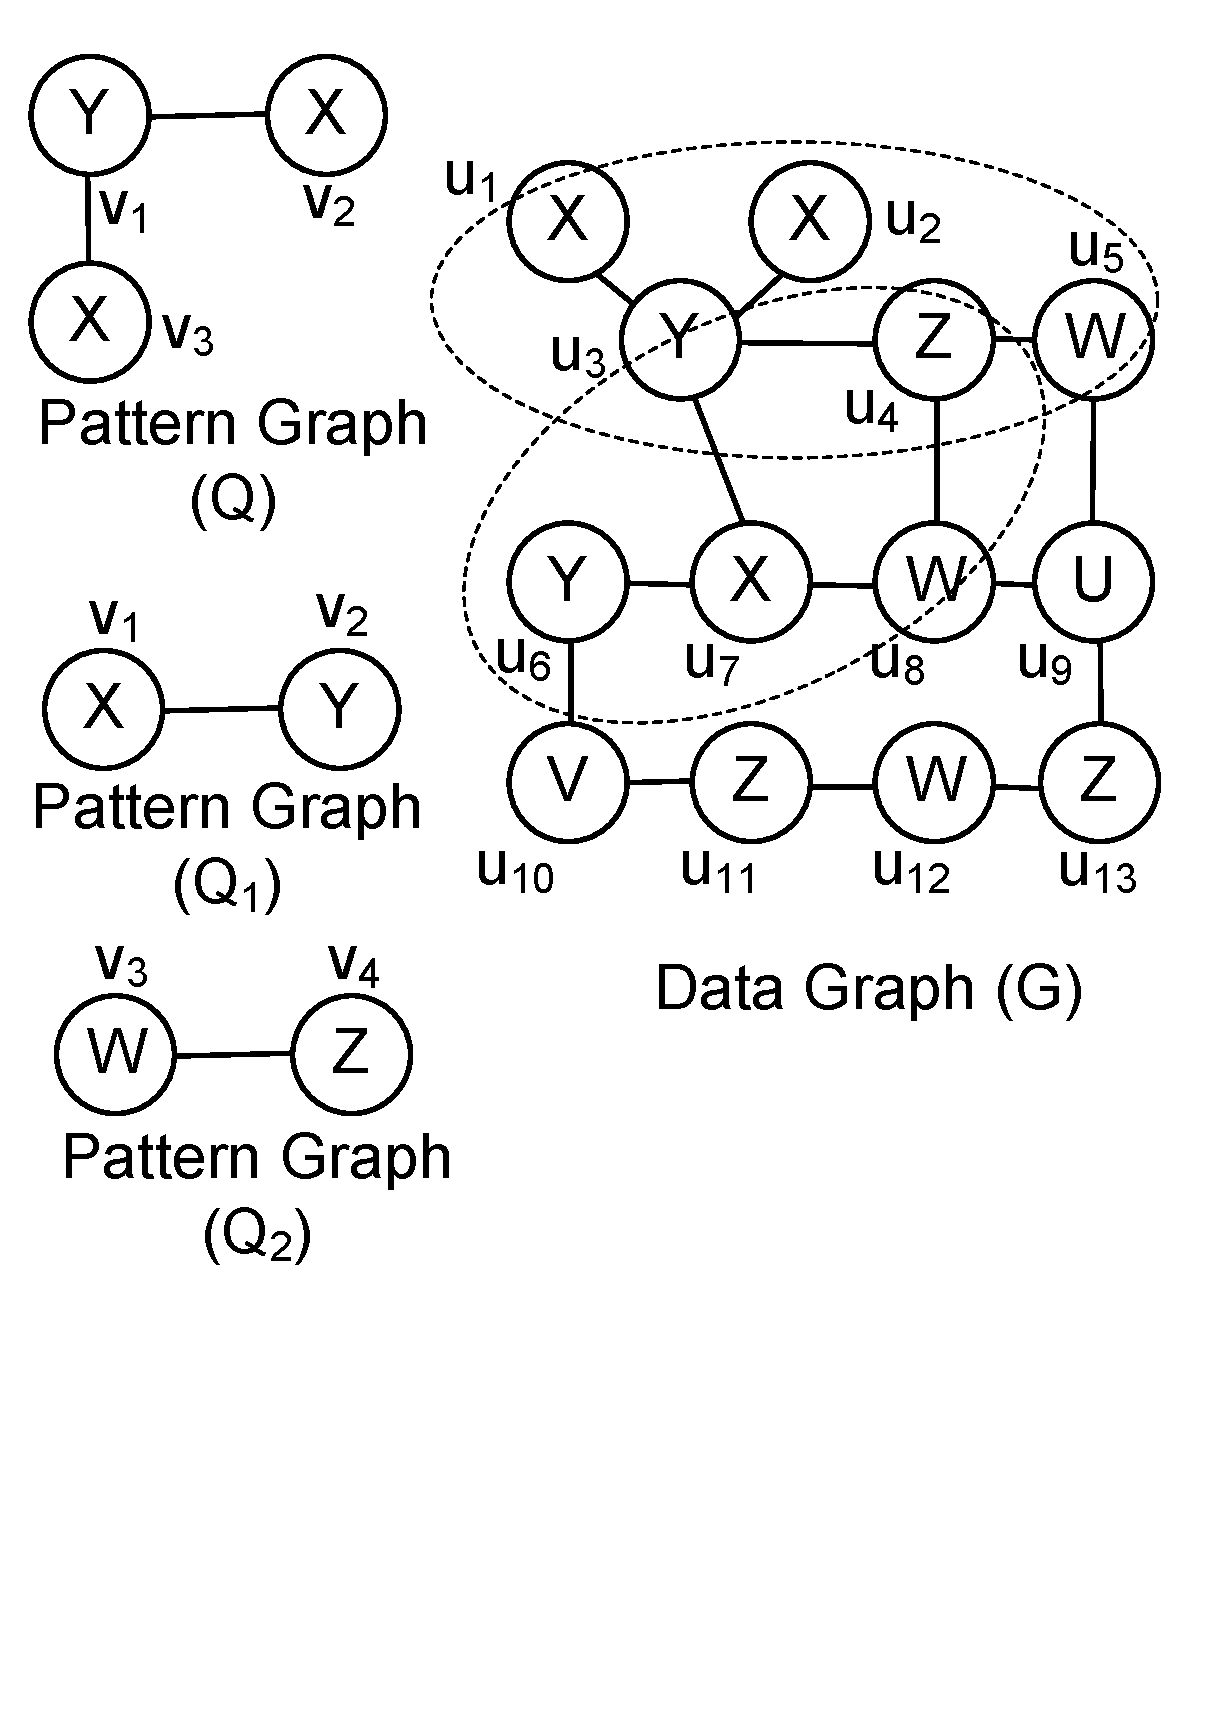
\includegraphics[scale=0.23]{images/correlation}
%\vspace{-1.75\baselineskip}
%\caption{Correlation between patterns $Q_1$ and $Q_2$ in $G$}
%\label{fig:correlation}
%\vspace{0.15\baselineskip}
%\end{figure}

Note that the grouping is not a partition of instances. It is possible for an instance
to belong to multiple groups, especially when the pattern has multiple nodes with the same label.
However, for a pattern $Q$, we ensure that the number of instance-groups would be $\sigma(Q)$.

Given two subgraph patterns $Q_1$ and $Q_2$, we compute their instance-groups:
$\mathbb{I'}=\{I'_1,I'_2,\ldots,I'_{\sigma(Q_1)}\}$ and $\mathbb{J'}=\{J'_1,J'_2,\ldots,$ $J'_{\sigma(Q_2)}\}$,
respectively. Without loss of generality, let us assume that $\sigma(Q_1) \le \sigma(Q_2)$.
Next, we count, out of all $\sigma(Q_1)$  instance-groups of $Q_1$, how many of them are ``close'' to at least
one instance-group of $Q_2$. We report this count as the {\em correlation} between $Q_1$ and $Q_2$ in $G$.
Finally, we define that two instance-groups $I' \in \mathbb{I'}$ and $J' \in \mathbb{J'}$
are close if there exist at least two nodes $u$ in $I'$ and $v$ in $J'$, such that their distance $d(u,v)\le h$,
that is, $u$ and $v$ are no more than $h$-hops away in the data graph $G$.
Clearly, $h\ge 0$ is a user-defined {\em distance threshold} parameter that can be varied to support different
amount of closeness between two co-occurrences of $Q_1$ and $Q_2$.
%
\begin{defn}[Correlation]
\label{def:correlation}
Given two patterns $Q_1$ and $Q_2$ in the data graph $G$, their instance-groups
$\mathbb{I'}=\{I'_1,I'_2,\ldots,$ $I'_{\sigma(Q_1)}\}$ and $\mathbb{J'}=\{J'_1,J'_2,\ldots,$ $J'_{\sigma(Q_2)}\}$,
respectively, and a user-defined distance threshold $h\ge0$,
assume that $\sigma(Q_1) \le \sigma(Q_2)$. We define the correlation
$\kappa(Q_1,Q_2,h)$ as:
%
\begin{align}
&\kappa(Q_1,Q_2,h) \nonumber & \\
&= |\{I' \in \mathbb{I'}:\exists J' \in \mathbb{J'}, \exists u \in I', \exists v \in J', d(u,v)\le h\}| \nonumber &
\end{align}
\end{defn}

The correlation, for the case $\sigma(Q_2) < \sigma(Q_1)$, can be defined analogously.
We note that the correlation between two subgraphs $Q_1$ and $Q_2$ is {\em symmetric}, that is,
$\kappa(Q_1,Q_2,h)$ = $\kappa(Q_2,Q_1,h)$.
%
\begin{exple}
Let us consider two subgraph patterns $Q_1$ and $Q_2$ in the data graph $G$ (Figure~\ref{fig:subgraph_isomorphism}),
and the distance threshold $h=1$. The instance-groups of $Q_1$ are given by: $\mathbb{I'}=\{u_1u_2u_7u_3,u_7u_6\}$,
where the groupings are performed based on the images of node $v_2$ in $Q_1$. Similarly,
the instance-groups of $Q_2$ are given by: $\mathbb{J'}=\{u_5u_4, u_8u_4,u_{11}u_{12}u_{13}\}$,
here the groupings are performed based on the images of node $v_3$ in $Q_2$. We have,
$\sigma(Q_1) =2 < \sigma(Q_2) =3$. Thus, we count, out
of two instance-groups of $Q_1$, how many of them are within $h=1$-hop of at least
one instance-group of $Q_2$. This gives us the correlation $\kappa(Q_1,Q_2,h=1)=2$.
\end{exple}

We are now ready to define our problem formally.
%
\begin{problem}
\label{prob:top-k}
{\bf {\sf Top-$k$} Correlated Subgraphs Mining (}{\sf{CSM}}{\bf).}
Given the data graph $G$, a user-defined distance threshold $h\ge0$, a minimum support threshold $\Sigma$, find the {\em top-$k$} pairs of subgraph patterns $\langle Q_1, Q_2 \rangle$ of $G$, having the
maximum correlations $\kappa(Q_1,Q_2,h)$, and for each subgraph pattern $\sigma(Q_1)\ge \Sigma$, $\sigma(Q_2)\ge \Sigma$.
\end{problem}

Analogous to the {\em association rule mining} over a transaction dataset \cite{AS94}, we consider both: {\bf (1)} a {\em minimum
support threshold} $\Sigma$ such that each constituent subgraph pattern is individually frequent, and {\bf (2)} a {\em correlation
measure} between a pair of frequent subgraph patterns so to identify the top-$k$ pairs based on their
correlations. Notice that {\bf (i)} if $Q_1$ is a subgraph of $Q_2$, or vice versa, the correlation between them is not interesting.
Thus in our methods, we remove those pairs which are related by subgraph and supergraph relationships.
Similarly, {{\bf (ii)} if $Q_1$ and $Q_2$ have high correlation {\em only} because they are subgraphs of a frequent
pattern $Q_3$, i.e., $Q_3 \succeq Q_1$ and $Q_3 \succeq Q_2$, such correlations are also not interesting. In our solution
framework, we devise a technique to detect and eliminate such subgraph pairs from our top-$k$ result.
%
%
\subsection{Theoretical Characterization}
\label{sec:characteristics}
%
The correlation metric satisfies several interesting properties.
%
\begin{lma}
\label{lemma:downward}
Correlation metric $\kappa(Q_1,Q_2,h)$ is not downward closure. Specifically, consider that $Q_3$ is a subgraph of $Q_2$, i.e.,
$Q_2 \succeq Q_3$. Then the following $\kappa(Q_1,Q_3,h) \ge \kappa(Q_1,Q_2,h)$ does not always hold.
\end{lma}
%
The downward closure property does not always hold because as one grows the size of the pattern (e.g., from $Q_3$ to $Q_2$), the super pattern
$Q_2$ may now have larger size instances that are closer to the instances of the other pattern $Q_1$.
In Figure~\ref{fig:subgraph_isomorphism}, let us consider
$Q_3$ as a single node with label $W$, whereas the patterns $Q_1$ and $Q_2$ are shown in the figure. Clearly, $Q_2 \succeq Q_3$.
We notice that $\kappa(Q_1,Q_3,h=1)=1$ and $\kappa(Q_1,Q_2,h=1)=2$. Hence, the downward closure property does not always hold.
%
\begin{lma}
\label{lemma:upward}
Correlation metric $\kappa(Q_1,Q_2,h)$ is not upward closure. In particular, consider that $Q_4$ is a supergraph of $Q_1$, i.e.,
$Q_4 \succeq Q_1$. Then the following $\kappa(Q_1,Q_2,h) \le \kappa(Q_4,Q_2,h)$ does not always hold.
\end{lma}
%
The upward closure property does not always hold because as one grows the size of the pattern (e.g., from $Q_1$ to $Q_4$), the super pattern
$Q_4$ may naturally have lower MNI support (and, hence smaller number of instance-groups).
This can reduce its correlation with the other pattern $Q_1$.
In Figure~\ref{fig:subgraph_isomorphism}, let us consider $Q_4$ consisting of three nodes $X-Y-X$,
whereas the patterns $Q_1$ and $Q_2$ are shown in the figure. Clearly, $Q_4 \succeq Q_1$.
We notice that $\kappa(Q_1,Q_2,h=1)=2$ and $\kappa(Q_4,Q_2,h=1)=1$. Hence, the upward closure property does not always hold.

Since upward and downward closure properties are widely used in frequent pattern mining problems \cite{AS94,KK01,BN08,FB07,KK04,YH02}
--- in particular, for early termination of the proposed algorithms, Lemma~\ref{lemma:downward} and \ref{lemma:upward} demonstrate the inherent
complexity of our {\sf{CSM}} problem.

Fortunately, Lemma~\ref{lemma:prune} would be useful to design an early termination criteria in our algorithm.
%
\begin{lma}
\label{lemma:prune}
The following inequality holds: $\kappa(Q_1,Q_2,h) \le \min \{\sigma(Q_1),\sigma(Q_2)\}$.
\end{lma}

Lemma~\ref{lemma:prune} directly follows from the definition of correlation (Definition~\ref{def:correlation}), which is computed
from the instance-groups of that subgraph pattern having the smaller support. 
\section{Exact Algorithm: {\sf CSM-E}}
\label{sec:exact_algo}
\begin{comment}
A Na\"{\i}ve approach to find the top-$k$ correlated pairs would be to {\bf (1)} first identify
all frequent subgraph patterns based on the minimum support threshold $\Sigma$ (e.g.,
via GRAMI \cite{EASK14}); {\bf (2)} enumerate all their instances in the data graph (e.g.,
via VF3 \cite{CarlettiFSV18}); {\bf (3)} compute correlation for every pair of frequent subgraph patterns;
and finally {\bf (4)} report the top-$k$ correlated pairs among them. However, this baseline method
is inefficient: Since we are interested in finding {\em only} the top-$k$ correlated pairs, computing
correlations for all pairs of frequent subgraph patterns would be expensive and also redundant.
\end{comment}
In this section, we design an {\em exact} and {\em holistic} algorithm, referred to
as {\sf CSM-E} (an abbreviation for Correlated Subgraphs Mining-Exact)
that follows {\em best-first exploration} of
frequent patterns, coupled with an {\em early termination} strategy, to report the top-$k$ correlated
subgraph pairs in a large network.
%
\subsection{Overview}
\label{sec:exact_algo_overview}
%
To find the relevant frequent patterns and the top-$k$ correlated pairs in a
holistic manner, we consider a {\em pattern search tree} $T$, whose $n$-th level
vertices \footnote{{\footnotesize To distinguish the nodes of the pattern search
tree $T$ from those of the data graph $G$, we use the notation ``vertices'' for
the pattern search tree.}} contain $n$-edge frequent subgraphs. In other words,
the first level of the pattern search tree consists of all frequent edges from
the data graph $G$. For any frequent subgraph in the pattern search tree, we use
{\em subscripts to label its nodes according to their discovery order}
\cite{YH02}. Thus, in a frequent subgraph in $T$, $i<j$ indicates that $v_i$ is
discovered before $v_j$. If there is an edge from $v_i$ to $v_j$ with $i<j$,
then it is called a {\em forward edge}; otherwise the edge is denoted as a {\em
backward edge}. We call $v_0$ the root and $v_n$ the rightmost vertex, where $n$
is the number of nodes in that frequent subgraph. The direct path (consisting
of forward edges only) from $v_0$ to $v_n$ is referred to as the {\em rightmost
path}.

To construct $(n+1)$-th layer from the $n$-th layer in the pattern search tree
$T$, a vertex in the $n$-th layer (which is a frequent subgraph, say $P$, from
$G$ having $n$ edges) is augmented with a new edge, and thus we create a new
subgraph, say $C$. We insert $C$ as a vertex in the $(n+1)$-th layer of $T$ if
and only if $C$ is also a frequent subgraph in $G$. We refer to $P$ as a {\em parent
vertex} and $C$ as its {\em child vertex} in $T$. Note that for an $n$-edge
graph, it may have $n$ different ways to be formed from $(n-1)$-edge graphs if
we do not consider isomorphism. The generation of {\em duplicate graphs} is
redundant and could affect the overall efficiency. To reduce the creation of
duplicate graphs, we follow the strategy developed in gSpan \cite{YH02}: {\em A
new edge can only grow from nodes along the rightmost path}. In
particular, {\bf (1)} backward edges can only grow from the rightmost node $v_n$
of $P$, while {\bf (2)} forward edges can grow from nodes on the rightmost path in
$P$. The {\em completeness guarantee} of generating all frequent subgraphs via
the aforementioned {\em rightmost extension} strategy can be found in
\cite{YH02}, and we omit the proof for brevity.

We note that the pattern search tree $T$ is not fully materialized, instead it
is built on demand. For example, gSpan \cite{YH02} explores $T$ in depth-first
manner; whereas in earlier apriori-based approaches (e.g., AGM \cite{IWM00} and
FSG \cite{KK01}) construct $T$ in breadth-first manner. However, we find that
neither depth-first exploration, nor breadth-first exploration is efficient for
our {\bf Top-$k$ Correlated Subgraphs} discovery problem. Rather, we propose a
novel {\em best-first exploration} algorithm, details of which are given in
\S~\ref{sec:bfe}.

Next, when a new frequent pattern $C$ is added in the pattern search tree $T$,
we compute $C$'s correlation with previously explored vertices in $T$ (i.e.,
frequent patterns from $G$ that have been discovered earlier than $C$). In
\S~\ref{sec:replica}, we discuss a memory-efficient data structure,
called $\mathcal{R}$eplica, to find correlation between a pair of frequent
subgraph patterns.

Finally, we employ a {\em priority queue} $\mathcal{Q}$ to store the top-$k$
correlation values (and the corresponding correlated subgraph pairs) found thus
far. In \S~\ref{sec:early_termination}, we further propose an {\em early
termination} strategy to speed up search, while returning the {\em
exact} top-$k$ correlated pairs upon termination.
This completes our algorithm.
%
\subsubsection{Best-First Exploration}
\label{sec:bfe}
%
A pair of subgraph patterns having individual higher support values can be
expected to have higher correlation between them. This is as such subgraph
patterns will have many instances which would likely be closer to each other in
the data graph $G$. Therefore, in the earlier stages of our algorithm, it is
more beneficial to consider patterns with higher support values; it can be
achieved via the best-first exploration of the pattern search tree. In
particular, let us denote by $\mathbb{P}$ the set of frequent patterns currently
in the pattern search tree $T$, whereas we represent by $\mathbb{C}$ the set of
their children that are frequent and also \emph{not} included in $T$. Among
all patterns in $\mathbb{C}$, we pick the one $C^*$ with the maximum support for
inclusion in $T$. We implement $\mathbb{C}$ as another \emph{priority queue} (referred
to as the {\em search queue} in our algorithm) to quickly extract $C^*$ from it.
Formally,
%
\begin{align}
& \mathbb{C}=\{C: \exists P \in T, C \, \text{is }P\text{'s child}, \sigma(C)\ge \Sigma, C \not\in T\} \nonumber & \\
& C^* =\arg\max_{C\in\mathbb{C}}\sigma(C) \nonumber &
\end{align}

If two or more patterns in $\mathbb{C}$ have the same maximum support, we add
one more condition in our best-first exploration: Among them, the pattern with
less number of edges is extracted earlier from $\mathbb{C}$}. This rule coupled
with the downward-closure property of the MNI support ensures that {\em all
subgraphs of $C^*$ must be included in $T$, before $C^*$ is extracted from the
search queue $\mathbb{C}$}.

We notice that unlike gSpan \cite{YH02}, depth-first exploration of the pattern search tree is not optimal in our case since
it identifies many subgraph-supergraph pairs at earlier stages, which are not useful for the {\bf Top-$k$ Correlated
Subgraphs} finding problem. On the other hand, breadth-first exploration is more memory intensive, and based on our
detailed empirical results in \S~\ref{sec:experiments}, it is still inefficient compared to our proposed
best-first exploration strategy.

\spara{Removing duplicates.} While the rightmost extension rules in gSpan
\cite{YH02} reduce the creation of duplicate graphs, it cannot entirely remove
them. To completely eliminate duplicated subgraphs, we further take advantage of
the {\em minimum DFS code} \cite{YH02}: whenever a subgraph $C^*$ is extracted
from $\mathbb{C}$, we compute its minimum DFS code, denoted as $MinDFS(C^*)$. We
also use a hash table $H$ to store all the minimum DFS codes for the vertices
(i.e., frequent subgraphs) already in $T$. When a new subgraph $C^*$ is
extracted, we perform a lookup for $MinDFS(C^*)$ in $H$. If found, then $C^*$
must have been discovered before, since two graphs will have the same minimum
DFS code if and only if they are isomorphic \cite{YH02}, therefore we do not
insert $C^*$ in $T$.
% via VF3 \cite{CarlettiFSV18}

\spara{Removing subgraph-supergraph pairs.} To avoid calculating correlations
between subgraph-supergraph pairs, we check if $C^*$ is a supergraph of already
included frequent patterns in $T$ by performing an explicit subgraph isomorphism
check between $C^*$ and every pattern $Q$ in $T$. Since practically $C^*$ and $Q$ are
small subgraphs and $T$ is also not exceptionally large, we find this to be an
inexpensive operation.
%
\subsubsection{Early Termination Criteria}
\label{sec:early_termination}
%
Our objective is to mine the top-$k$ pairs of correlated (frequent) subgraphs,
and ensure that some other pair of frequent subgraphs cannot have a higher
correlation $(\kappa)$ than any pair in our {\sf Top-$k$} {\em priority queue}
$\mathcal{Q}$. A closer look at Lemma~\ref{lemma:prune} mentioned in
\S~\ref{sec:characteristics} allows us to deduce the following. Consider that
$C^*$ is the current frequent subgraph extracted from $\mathbb{C}$. By
Lemma~\ref{lemma:prune}, $\kappa(C^*,Q,h)\le \sigma(C^*)$, for all frequent
subgraphs $Q$ already in the pattern search tree $T$. Moreover, for any other
pattern $C_1$ that would be added in $T$ after $C^*$,
$\sigma(C_1)\le\sigma(C^*)$ due to best-first exploration thereby resulting in
$\kappa(C_1,Q,h)\le \sigma(C_1) \le \sigma(C^*)$, for all $Q$ in $T$. Hence, if
$\sigma(C^*)$ is lower than the least correlation value ($\kappa$) currently
stored in $\mathcal{Q}$, while $\mathcal{Q}$ being full, we can safely terminate
our search, and report the subgraph pairs in $\mathcal{Q}$ as our exact
solution set.

It is also possible that $k$ correlated pairs do not even exist in the data graph $G$,
given some higher minimum support threshold $\Sigma$ and larger values of $k$. In this case, the {\em priority queue} $\mathcal{Q}$
will never get full, and yet there would not exist any more frequent subgraph to
include in $T$. Thus, we terminate our algorithm.
%
%
\begin{algorithm}[tb!]
{\scriptsize
 \dontprintsemicolon
 \caption{\textsc{Mining Top-$k$ Correlated Pairs}}
 \label{algo:exact}
 \nonl \textbf{Input:} data graph $G=(V,E,L)$, minimum support threshold $\Sigma$,
 distance threshold $h\ge0$, positive integer $k$ \;
 \nonl \textbf{Output:} Top-$k$ pairs of correlated patterns \emph{s.t.} each
 pattern has support $\ge \Sigma$  \;
 Initialize {\sf Pattern Search Tree} $T\leftarrow\ \emptyset$ \;
 Initialize {\sf Search Queue} $\mathbb{C} \leftarrow ${\sf\ Frequent Edges} in $G$\;
 Initialize {\sf Hash Table} $H\leftarrow\ \emptyset$ \; %\COMMENT{stores {\sf Min DFS Codes} of subgraphs in $T$} \;
 Initialize {\sf Priority Queue} $\mathcal{Q}\leftarrow\ \emptyset$ with maximum size $k$ \; %\COMMENT{stores {\sf Top-$k$ Correlated Pairs} found so far} \;
 \While(\tcp*[h]Search){\textup{$\mathbb{C}$ is non-empty}}
 {
   Pattern $C^* \leftarrow$ {\sf Best-First-Pop($\mathbb{C}$)} (\S~\ref{sec:bfe}) \;
   \If {\textup{\textsc{Termination Condition} (\S~\ref{sec:early_termination}) is {\sf True}}}
   {
     Goto Line 19 \;
   }
   \If {\textup{$MinDFS(C^*)  \not\in H$}}
   {
       \lIf {\textup{$\exists \langle Q_1,Q_2 \rangle \in \mathcal{Q}, \kappa(Q_1,Q_2,h)=\sigma(C^*), C^*\succeq Q_1,Q_2$ }}
       {
         Remove $\langle Q_1,Q_2 \rangle$ from $\mathcal{Q}$ \;
       }
       \ForEach{\textup{$Q\in T$}}
       {
         \If {\textup{$Q$ is not a subgraph of $C^*$}}
         {
            Compute correlation $\kappa(C^{*},Q,h)$ (\S~\ref{sec:replica})\;
            Insert $\kappa(Q_1,Q_2,h)$ in $\mathcal{Q}$ (if necessary) \;
         }
       }
       Insert $C^*$ in $T$, $MinDFS(C^*)$ in $H$ \;
      %  Insert
	   \makebox[\linewidth][l]{Find {\sf Children}$(C^*)$ via {\sf Rightmost Extension} (\S~\ref{sec:exact_algo_overview})}\;
	% \makebox[\linewidth][l]{{\sf Children}$(C^*)$ $\leftarrow Extend(C*) {\sf Rightmost Extension} (\S~\ref{sec:exact_algo_overview})}\;
       \ForEach{\textup{{\sf Child}$ \in {\sf Children}(C^*)$}}
       {
         \lIf {\textup{$\sigma$({\sf Child})$\ge\Sigma$}}
         {
           Insert {\sf Child} in $\mathbb{C}$ \;
         }
       }
   }
 }
 \Return {\textup{Top-$k$ correlated pairs currently in $\mathcal{Q}$}}\;}
\end{algorithm}
%

\spara{Removing subgraph pairs with high correlation only due
to a frequent supergraph.} We now turn our attention to the problem of
disregarding subgraph pairs $Q_1$ and $Q_2$
from our top-$k$ priority queue when the pair has high correlation {\em only} because both $Q_1$ and $Q_2$ are
subgraphs of another frequent pattern $C^*$, i.e., $C^* \succeq Q_1$ and $C^* \succeq Q_2$.

In particular, we are concerned when the supergraph $C^*$ of both $Q_1$ and
$Q_2$ has the same support as the correlation between $Q_1$ and $Q_2$, where the
pair $Q_1,Q_2$ is currently in the top-$k$ priority queue $\mathcal{Q}$. Since
$\sigma(C^*)=\kappa(Q_1,Q_2,h)$, and the pair $Q_1,Q_2$ is in $\mathcal{Q}$, the
termination criteria of our algorithm will not be satisfied. Next, to remove the
pair $Q_1,Q_2$ from $\mathcal{Q}$, we incorporate the following procedure in our
mining algorithm: every time a new pattern $C^*$ is extracted from the search
queue $\mathbb{C}$, if the termination criteria is not satisfied, we check if
there exists a correlated pair $Q_1,Q_2$ in $\mathcal{Q}$, such that both $Q_1$
and $Q_2$ are subgraphs of $C^*$ and $\sigma(C^*)=\kappa(Q_1,Q_2,h)$, in
which case we eliminate the pair $Q_1,Q_2$ from $\mathcal{Q}$.

\subsubsection{Putting Everything Together}
\label{sec:exact_description}
%
Our pipeline is described in Algorithm~\ref{algo:exact}.
It begins with finding all frequent edges in data graph $G$,
which are then queued in the search queue $\mathbb{C}$
following a frequency-determined priority ordering (Line 2).
\textit{Search} begins and continues as long as $\mathbb{C}$ contains queued patterns
and the termination condition is unsatisfied (Lines 5-18).
$C^{*}$, selected as the best-first choice
from $\mathbb{C}$, is processed for correlation (\S~\ref{sec:cor_compute}) with every other
previously explored pattern $Q$ in search tree $T$ subject to satisfaction of
constraints described in \S~\ref{sec:bfe}, \ref{sec:early_termination} (Lines 6-13). Top-$k$ priority queue is updated
based on the computed $\kappa$ values (Line 14). $C^{*}$ is then inserted in $T$ and its
minimum {\sf DFS Code} is inserted in $H$ (Line 15), followed by the extension of $C^{*}$ to generate
its \emph{child} patterns. All frequent children of $C^{*}$ are inserted
in $\mathbb{C}$ for future processing and the loop continues (Lines 16-18).
Upon termination, the algorithm returns Top-$k$ pairs of correlated subgraph (Line 19).
%
\subsection{Storing Subgraph Instances: The $\mathbfcal{R}$eplica}
\label{sec:replica}
%
We now focus on the problem of correlation computation between two subgraph patterns
which requires enumerating and finding distances between every pair of instances for
both these patterns. This is memory intensive and computationally demanding due to the
following reasons: {\bf (1)} Storing all instances of all frequent subgraphs discovered so far
can easily overwhelm the memory. We notice that for the frequent
subgraph mining algorithms, e.g., in gSpan \cite{YH02} and GraMi \cite{EASK14},
storing all instances of all discovered frequent patterns is not required.
This illustrates an additional challenge of our problem. {\bf (2)} Many
redundant distance computations could take place: assume two instances
$I_1$ and $I_2$ for patterns $Q_1$ and $Q_2$ respectively, are within $h$-hops
in $G$. Consider a superpattern $Q_3 \succeq Q_1$, and $I_3$, which is extended from $I_1$, is an
instance of $Q_3$. To compute correlation between $Q_3$ and $Q_2$,
verifying the distance between their instance pairs $I_3$ and $I_2$ respectively
is redundant, since
it is guaranteed that they would also be within $h$-hops in $G$.

We solve both these challenges with an efficient data structure, called $\mathcal{R}$eplica
that stores all instances of a subgraph pattern in a compressed manner (\S~\ref{sec:rep_data}).
Our $\mathcal{R}$eplica structure also helps quickly generate instances of a superpattern
extended from a parent pattern (\S~\ref{sec:rep_generate}). Moreover, we design an {\em incremental distance
indexing} method (\S~\ref{sec:index}) that permits deletion of $\mathcal{R}$eplicas of those patterns in $T$
for which all their frequent children patterns (obtained via rightmost extension) have also
been included in $T$. In other words, at any point in our algorithm, we only store $\mathcal{R}$eplicas for the 
following patterns: {\bf (1)} The pattern $C^*$ that is currently extracted from the search queue $\mathcal{Q}$
(Line 6, Algorithm~\ref{algo:exact}), and {\bf (2)} {\em only} those patterns in $T$ for which they have at least one child
in the search queue $\mathbb{C}$. This greatly facilitates in reducing memory footprints 
and redundant distance computations. Finally, we introduce the
correlation computation strategy in \S~\ref{sec:cor_compute}.
%
\subsubsection{$\mathcal{R}$eplica Data Structure}
\label{sec:rep_data}
%
Given the data graph $G$ and a pattern $Q=(V_Q,E_Q,L)$, $\mathcal{R}$eplica$(Q)=(V_{\mathcal{R}(Q)},E_{\mathcal{R}(Q)},L)$ is a subgraph of $G$,
constructed by the {\em graph-union}
\footnote{{\footnotesize The union $\mathcal{G} = \mathcal{G}_1 \cup \mathcal{G}_2$ of graphs $\mathcal{G}_1=(V_1,E_1,L)$
and $\mathcal{G}_2=(V_2,E_2,L)$ is $\mathcal{G} = (V_1\cup V_2, E_1\cup E_2,L)$.}}
of all instances of $Q$ in $G$. Since $\mathcal{R}$eplica$(Q)$ is a subgraph, it is stored as an adjacency list in the memory.

In addition to the aforementioned graph, we store two kinds of node mappings as follows:

\spara{Forward Node Mapping.} $\forall u \in  V_Q$, forward node mapping $Mapping(u,\mathcal{R}\text{eplica}(Q))$
stores all nodes $v\in V_{\mathcal{R}(Q)}$,
such that $v$ is a mapping of $u$ in some instance $I$ of $Q$ within $\mathcal{R}$eplica$(Q)$.

\spara{Inverse Node Mapping.}  $\forall v \in V_{\mathcal{R}(Q)}$, inverse node mapping
$Mapping^{-1}$ $(v, Q)$ stores the set of all $u\in V_Q$ such
that $v\in Mapping(u,\mathcal{R}\text{eplica}(Q))$.

$\mathcal{R}$eplica provides a middle-ground compared to two extreme alternatives: {\bf (1)}
{\em explicitly} store all instances of all generated patterns \cite{KK04}, or {\bf (2)} enumerate all instances
of a pattern whenever required (in runtime) from the {\em large} data graph $G$. In contrast to these alternatives,
the {\em $\mathcal{R}$eplica is economical from both storage and efficiency point of view: it not only avoids
potential memory requirement issues by {\em implicitly} storing
all instances of a pattern, but also lays a robust foundation for carrying out
efficient correlation calculations that we shall discuss in \S~\ref{sec:cor_compute}}.

Note that both forward and inverse node mappings can be deduced from the
$\mathcal{R}$eplica$(Q)$ subgraph via subgraph isomorphism with the pattern $Q$.
However, we explicitly maintain these mappings for computational efficiency:
Forward Node Mapping allows us to readily compute $\sigma(Q)$ and also assists
in $\mathcal{R}$eplica generation, while the Inverse Node Mapping enables us to
quickly prune candidate nodes of $\mathcal{R}$eplica$(Q)$ for matching with a
node in $Q$ while performing isomorphism. The utility of using these mappings
will become apparent in \S~\ref{sec:rep_generate}.
%
\subsubsection{On-Demand Replica Generation for a New Pattern}
\label{sec:rep_generate}
%
\begin{algorithm} [tb!]
 \caption{\textsc{Build Replica for a New Pattern}}
 \label{algo:getreplica}
{\scriptsize
 \dontprintsemicolon
 \nonl \textbf{Input:} data graph $G=(V,E,L)$, parent
 pattern $Q=(V_Q,E_Q,$ $L)$, $\mathcal{R}$eplica$(Q)=(V_{\mathcal{R}(Q)}$,
 $E_{\mathcal{R}(Q)}$, $L)$, child pattern $R=(V_R$, $E_R$, $L)$, extending node:
 $u\in V_Q$, extending edge: $(u,v) \in E_R$ \;
\nonl \textbf{Output:} $\mathcal{R}$eplica$(R)$ \;
	\vspace{0.3mm}
	$DFS\ List(Q)\leftarrow$ get edge list via rooted DFS in $Q$ with $u$ as root \;
	Initialize $instance \leftarrow \emptyset, $ $ \mathbb{I} \leftarrow \emptyset$\;
	\ForEach{ $u' \in Mapping(u,\ \mathcal{R}$\textup{eplica}$(Q))$}
	{
		$instance.{\sf add}(u\mapsto u')$\;
		\ForEach{\textup{edge} $(u',v')\in E_G$ \textup{that maps to the extending edge} $(u,v)\in E_R$}
		{
			$instance.{\sf add}(v\mapsto v')$\;
	        $\mathbb{I}\leftarrow$ \textsc{FindAllInstances($G$, $Q$, $\mathcal{R}eplica(Q)$, $R$,
	        $DFS\ List(Q)$, $instance$, $\mathbb{I}$)}\;
			\textsc{UpdateReplica($R$, $\mathcal{R}eplica(R)$, $\mathbb{I}$)}\;
			% $instance\leftarrow instance \setminus \{(v,v')\}$\;
			$instance.{\sf delete}(v\mapsto v')$\;
		}
		% $instance\leftarrow instance \setminus \{(u,u')\}$\;
		$instance.{\sf delete}(u\mapsto u')$\;
	}	
	\Return{$\mathcal{R}$\textup{eplica}$(R)$}\;}
\end{algorithm}
%
\vspace{-2mm}
\begin{algorithm}[tb!]
 \caption{\textsc{FindAllInstances:Exact Method}}
 \label{algo:findallinstances}
{\scriptsize
 \dontprintsemicolon
 \nonl \textbf{Input:} data graph $G=(V,E,L)$, parent
 pattern $Q=(V_Q,E_Q,$ $L)$, $\mathcal{R}$eplica$(Q)=(V_{\mathcal{R}(Q)}$,
 $E_{\mathcal{R}(Q)}$, $L)$, child pattern $R=(V_R$, $E_R$, $L)$,
    $DFS\ List(Q)$, partial isomorphism of $R$: $instance$, $\mathbb{I}$\;
\nonl \textbf{Output:} $\mathbb{I}: $ set of all instances of $R$ in $G$ consistent with input partial isomorphism $instance$\;
	\uIf{$instance$ \textup{is} {\sf Found}}
	{
		\Return{$\{instance\}$}
	}
	\Else
	{
		$e=(p,c)\leftarrow$ \textsc{NextQueryEdge($DFS\ List(Q)$)}\;
		$v' \leftarrow instance(p)$\;
		\uIf{$e$ \textup{is a} {\sf backward edge}}
		{
			\uIf{\textup{an edge} $(v',instance(c))$ \textup{exists in} $E_{\mathcal{R}(Q)}$}
			{
				$\mathbb{I} \leftarrow \mathbb{I}\ \cup$ \textsc{FindAllInstances({$G$}, $Q$, $\mathcal{R}eplica(Q)$, $R$, $DFS\ List(Q)$, $instance$, $\mathbb{I}$)}\;
			}
			\Else{\Return $\emptyset$}
		}
		% (\tcp*[h]{{$e$ is a forward edge}})
		\Else{
		$P_{c} \leftarrow$ \textsc{FilterCandidates($v'$, $c$, $Q$, $\mathcal{R}eplica(Q)$)}\;
		\ForEach{$w' \in P_{c}$ s.t. \textup{$w'$ is not matched in} $instance$}
		{
		%   $instance \leftarrow instance \cup \{(c,w')\}$\;
			$instance.{\sf add}(c\mapsto w')$\;
			$\mathbb{I} \leftarrow \mathbb{I}\ \cup$ \textsc{FindAllInstances({$G$}, $Q$, $\mathcal{R}eplica(Q)$, $R$, $DFS\ List(Q)$, $instance$, $\mathbb{I}$)}\;
		% $instance \leftarrow instance \setminus \{(c,w')\}$\;
			$instance.{\sf delete}(c\mapsto w')$\;
		  }}
		\Return{$\mathbb{I}$}\;
	}}
\end{algorithm}
%
%
We create $\mathcal{R}$eplicas in an incremental manner: given $\mathcal{R}$eplica$(Q)$ of a parent
pattern $Q$, we generate $\mathcal{R}$eplica$(R)$ of its child pattern $R$. Our exact approach for
replica extension is given in Algorithm~\ref{algo:getreplica}, which essentially describes a backtracking
procedure for subgraph isomorphism similar to the {\em Ullman's algorithm} \cite{U76}.


Algorithm \ref{algo:getreplica} begins with a depth-first search ({\sf DFS}) procedure (Line 1)
executed on parent $Q$, selecting $u\in V_{Q}$ at which the
\emph{extending edge} $(u,v)$ is grown as the \emph{root}. We call $u$ the
\textit{extending node}. Both forward and backward edges encountered in the {\sf DFS}
starting at $u$ are recorded in an ordered list called the \emph{DFS List},
which guides the isomorphism performed subsequently. For every mapping $u'$ of
$u$ in $\mathcal{R}$eplica$(Q)$, the algorithm attempts to enumerate all
instances of child $R$ in $G$ fixing $u\mapsto u'$ (Lines 3-10). It does so by matching $v$
next, the newly extended node to all nodes $v'\in V$ adjacent to $u'$,
such that edge $(u',v')\in E$ is a valid mapping for $(u,v)\in E_{R}$ (Lines 5-6). It
then invokes \textsc{FindAllInstances} (Algorithm \ref{algo:findallinstances})
which uses $\mathcal{R}$eplica$(Q)$ to find every instance of $R$ such that
$u\mapsto u'$ and $v\mapsto v'$ (Line 7).

Algorithm \ref{algo:findallinstances}, as invoked above, recursively enumerates all instances
of $R$ in a depth-first manner following \emph{DFS List(Q)}. In the general case (Lines 4-17), the algorithm
begins by invoking \textsc{NextQueryEdge} which returns one edge at a time from
$E_{Q}$ in the order of \emph{DFS List(Q)}. Edge $e=(p,c)$, thus returned, connects
nodes $p,c \in V_Q$ such that $c$ is the pattern node to be matched next; $p$ is already
matched to $v' \in V_{\mathcal{R}(Q)}$. (The first call to
Algorithm \ref{algo:findallinstances} in every iteration of the inner loop in
Algorithm \ref{algo:getreplica} always has $p$ matched with $u'$).
If, however, $e$ is a backward edge, $c$ is already matched in which case the
algorithm checks whether an edge exists in $\mathcal{R}$eplica$(Q)$
connecting $v'$ and $instance(c)$: if it does exist, it proceeds with the
search for the next node matching, but returns unsuccessfully if it does not. If
$e$ is a forward edge, the algorithm calls \textsc{FilterCandidates} to compute the candidates set $P_c$ for storing
all nodes $w'\in V_{\mathcal{R}(Q)}$ for matching $c$ such that:
\textbf{(1)} $w'$ is a neighbor of $v'$ in $\mathcal{R}$eplica(Q); \textbf{(2)}
$c$ exists in the Inverse node mapping set for $w'$ in $\mathcal{R}$eplica(Q). That
is,
%$\forall$ $w' \in P_{c}$,
$c\in Mapping^{-1}(w', Q)$;
%\textbf{(3)} Edge label of $(v',w')\in E_{\mathcal{R}(Q)}$ matches that of $(p,c)\in E_Q$.
Next, for every node $w' \in P_{c}$ such that $w'$ has not already been matched in the
current \textit{instance}, the algorithm attempts the match $c\mapsto w'$ in \textit{instance}
and recursively calls \textsc{FindAllInstances} to match
remaining pattern nodes following the edges in \textit{DFS List}. \textit{Base
case} (Lines 1-2) occurs when the algorithm finds an \textit{instance} of $R$,
which it simply returns.

The set of all instances $\mathbb{I}$ thus found is returned by Algorithm \ref{algo:findallinstances} (Line 17) and is recorded by
Algorithm \ref{algo:getreplica}. In \textsc{UpdateReplica} (Algorithm \ref{algo:getreplica}, Line 8), the algorithm
updates $\mathcal{R}$eplica$(R)$ by performing a graph union with all instances in $\mathbb{I}$. It also updates the
\textit{Mappings} and \textit{Mappings$^{-1}$} indices to record new mappings found for every $instance$ in $\mathbb{I}$.
%
%This $\mathcal{R}$eplica-based instance storage strategy not only builds a foundation for an
%efficient correlation calculations, but also benefits the MNI support counting in
%the single large graph since we can directly get $\sigma(R)$ by counting all the sizes of the $Mapping(v)$, $v\in
%V_Q$.
%
%
%
\begin{figure}[t]
	\captionsetup{textfont=bf,font=small}
	\captionsetup[subfigure]{font=small, skip=-1pt}
	\begin{subfigure}[b]{0.5\textwidth}
		\centering
		\includegraphics[scale=0.5]{img_ex/G.pdf}\hspace*{2.5em}
		\caption{data graph $G$}
		\label{fig:exactG}
	\end{subfigure}%

    \begin{subfigure}[b]{0.15\textwidth}
            % \centering
            \hspace{4mm}\includegraphics[scale=0.5]{img_ex/patternQ.pdf}
            \caption{Parent $Q$}
			\label{fig:exact-Q}
    \end{subfigure}%
    \hspace*{\fill}
    % \captionsetup[subfigure]{labelfont=bf,textfont=normalfont,singlelinecheck=on,justification=raggedright, skip=-5pt}
	\begin{subfigure}[b]{0.3\textwidth}
            % \centering
            \hspace{-2.5mm}\includegraphics[scale=0.5]{img_ex/replicaQ.pdf}
            \caption{$\mathcal{R}$eplica$(Q)$}
			\label{fig:exact-REPQ}
	\end{subfigure}

	% \captionsetup[subfigure]{skip=-2pt}
	\begin{subfigure}[b]{0.15\textwidth}
		% \centering
		\hspace{4mm}\includegraphics[scale=0.5]{img_ex/patternR.pdf}
		\caption{Child $R$}
		\label{fig:exact-R}
	\end{subfigure}%
	\hspace*{\fill}
	\begin{subfigure}[b]{0.3\textwidth}
		% \centering
		\hspace{0mm}\includegraphics[scale=0.5]{img_ex/replicaR.pdf}
		\vspace{-0.25mm}
		% \vspace{-1.3\baselineskip} %not needed because figures are aligned
		% naturally unline above case
		\caption{$\mathcal{R}$eplica$(R)$}
		\label{fig:exact-REPR}
	\end{subfigure}
	% \captionsetup[figure]{skip=200pt}
    % \vspace{-1.75\baselineskip}
	\caption{$\mathcal{R}$eplica generation for a new subgraph pattern}
	\label{fig:exact-EX}
	% \vspace{0.15\baselineskip}
\end{figure}
%
%
\begin{exple}
Initially, $Q$ and $\mathcal{R}$eplica$(Q)$ are shown in Figs. \ref{fig:exact-Q}
and \ref{fig:exact-REPQ}, respectively. Child $R$, extended from $Q$ at
\emph{extending node} $s_0$ using the \emph{extending edge} $(s_0, s_3)$ is
given in Figure \ref{fig:exact-R}. Assume \emph{DFS List} for \emph{DFS}
starting at $s_0$ records edges $(s_0, s_1)$ and $(s_0, s_2)$ in that order. To
construct $\mathcal{R}$eplica$(R)$, the algorithm iterates over
$Mapping(s_0,\mathcal{R}$eplica$(Q))$, i.e. set $\{v_0, v_1\}$. With $s_0\mapsto
v_0$, the algorithm then considers vertices in $G$ (Fig. \ref{fig:exactG}) for
matching $s_3$. Thus, for each of $s_3\mapsto \{v_2, v_3\}$, the algorithm makes
recursive invocations to map $s_1$ and $s_2$ following the \emph{DFS List}
thus successfully enumerating instances. With $s_0\mapsto v_1$ however, no
mappings for matching $s_3$ exist. Graph union of all instances of $R$ thus
enumerated results in $\mathcal{R}$eplica$(R)$ depicted in Fig. \ref{fig:exact-REPR}.
% Assume, $(V_0, V_6), (V_0, V_7)\in E(G)$ map to $(A, D)$; but no such
% mapping edges exist incident to $V_1$ in $G$. All instances of $R$ thus found
% would result in $\mathcal{R}$eplica$(R)$ depicted in Figure \ref{fig:exactrepr}.
%
\end{exple}
%
\subsubsection{Indexing to Facilitate $\mathcal{R}$eplica Deletion of Old Patterns}
\label{sec:index}
%
We build and maintain two distance-based indexes, which permit us deleting $\mathcal{R}$eplicas of old
patterns once all their frequent children patterns (via rightmost extension) have been 
included in the pattern search tree $T$.

% \squishlist
\spara{\bf Proximity Nodes.} For each frequent node $u$ in data graph $G$, we
store proximity nodes of $u$ that are also frequent, denoted as $CorV(u)$: for
each node $v\in CorV(u)$, it holds that $d(u,v)\le h$.
% \squishend
% \squishlist

\spara{\bf Proximity Patterns.} For each frequent node $u$ in $G$, we store
patterns that are already included in $T$ and are within distance $h$ from
$u$. This is denoted as $CorP(u)$. For each pattern $Q\in CorP(u)$, {\bf (1)}
$Q\in T$, and {\bf (2)} given the instance-groups
$\mathbb{I'}=\{I'_1,I'_2,\ldots,I'_{\sigma(Q)}\}$ of $Q$, $\exists I'\in
\mathbb{I'}$, $\exists v\in I'$, it holds that $d(u,v)\le h$.
% \squishend

The {\em proximity nodes index} ($CorV$) is constructed before our mining
process starts, while the {\em proximity patterns index} ($CorP$) is updated
incrementally every time a new pattern $Q$ is inserted in the pattern search
tree $T$. The details of $CorP$ maintenance will be discussed in
\S~\ref{sec:cor_compute}. Since we already have $h$-hop proximity information
about all existing patterns in $T$, it allows us to delete their $\mathcal{R}$eplica
structures, thereby reducing the memory footprint of our technique.
%
%
\subsubsection{Correlation Computation}
\label{sec:cor_compute}
%
We recall that when a pattern $C$ is extracted from the search queue $\mathcal{Q}$, its
correlation is calculated with every pattern already in the pattern search tree $T$.
In the following, we focus on the computation of correlation $\kappa(C,Q,h)$ between $C$ and some $Q\in T$.
Due to our best-first exploration strategy, $\sigma(C)\le\sigma(Q)$, thus we need to verify
for every instance-group $I'$ of $C$, if there is some instance-group of $Q$ within distance $h$.

First, to find all instance-groups of $C$, our novel data structure $\mathcal{R}$eplica$(C)$ would be
immediately useful: Forward node mapping allows us to readily compute the MNI support of $C$, and the
node $v$ in $C$ having the minimum MNI support. For every $u \in Mapping(v,\mathcal{R}\text{eplica}(C))$,
we enumerate from $\mathcal{R}$eplica$(C)$ all instances of $C$ having $u$ (Algorithm~\ref{algo:findallinstances}).
This generates the instance-group of $C$ containing $u$. In this way, one can also efficiently enumerate all instance-groups
of $C$.

Given an instance-group $I'$ of $C$, we find if any instance-group of $Q$ is  within distance $h$ from $I'$ as demonstrated below.
Consider $CorP(w)$ for all node $w \in I'$. If $\cup_{w \in I'} CorP(w)$ contains $Q$, this essentially indicates that
there is some instance-group of $Q$ within distance $h$ from $I'$.
Ultimately, we count, out of all $\sigma(C)$ instance-groups
of $C$, how many of them are close to at least one instance-group of $Q$.
This count is reported as the correlation $\kappa(C,Q,h)$.
In this way, our {\em proximity nodes index} ($CorP$)
aids in efficient correlation computation.

\spara{Incrementally Updating Proximity Patterns Index.} Finally,
we incrementally update the $CorP$ index as follows. If $CorV(w)$ contains $u$ for some $w\in I'$, we include
the new pattern $C$ in $CorP(u)$. Thus, we also ensure that at any point in our algorithm, $CorP(u)$ would
contain all patterns in $T$ which are within distance $h$ from $u$.
%
%
\subsection{Complexity Analysis}
\label{sec:complexity_exact}
%
For simplicity, we use the notations below:
The data graph $G$ has $n$ nodes and $m$ edges,
among them $n_f$ nodes and $m_f$ edges are frequent based on the input
minimum support threshold. We denote by $n_h$ and $m_h$ the maximum number
of nodes and edges in the $h$-hop of a node in $G$. The pattern search tree
$T$ has at most $n_T$ vertices, with $n'_T$ vertices having at least one frequent child in the search queue $\mathcal{C}$, during the execution of our algorithm. Let the maximum number of nodes and
edges in a pattern $Q$ mined by our method be $n_Q$ and $m_Q$, and those in a replica be
$n_{\mathcal{R}}$ and $m_{\mathcal{R}}$, respectively. Finally,
also assume that the maximum size of the forward node mapping set be $M$
for some node in a frequent pattern mined by our algorithm.
%
\subsubsection{Time Complexity}
We start with the complexity analysis of {\em replica creation} for a new pattern $Q$ (\S~\ref{sec:rep_generate}).
For every mapping of the {\em extending edge} in $G$, we enumerate all possible
instances of $Q$ using the replica subgraph of its parent pattern. There can be $\bigO(m)$
matches for the extending edge, whereas the complexity of enumerating all possible
instances of $Q$ using the parent's replica is bounded by $\bigO(M^{n_Q})$. Hence,
the time complexity of building the replica of $Q$ is $\bigO(mM^{n_Q})$.

The creation of  {\em proximity nodes index} (\S~\ref{sec:index})
requires $h$-hop BFS from every frequent node in $G$,
and hence it has total time complexity: $\bigO(n_f(n_h+m_h))$. In contrast, whenever a new frequent
pattern is mined, one requires updating the {\em proximity patterns index}. This is performed
by traversing every node in the replica of the new pattern, and then finding their $h$-hop frequent
nodes using the proximity nodes index --- this has time complexity $\bigO(n_{\mathcal{R}}n_f)$. Since the pattern search tree
$T$ has at most $n_T$ vertices, total time complexity due to updating of proximity patterns index is
given by $\bigO(n_{\mathcal{R}} n_f n_T)$.

Correlation computation (\S~\ref{sec:cor_compute}) between the new pattern $Q$ extracted from the search queue $\mathbb{C}$
and an existing pattern in $T$ is essentially bounded by the complexity of enumerating all instances of $Q$ in its replica, i.e., $\bigO(M^{n_Q})$.
Since $T$ has at most $n_T$ patterns, one performs $\bigO(n_T^2)$ correlation computations, which has time
complexity $\bigO(n_T^2 M^{n_Q})$.

Considering all above, the time complexity of our exact algorithm, {\sf CSM-E}
\footnote{{\footnotesize We neglected times required for finding the best pattern
from search queue $\mathbb{C}$, verifying its subgraph relationships
with existing patterns in $T$, and computing its rightmost extensions,
due to relatively smaller sizes of frequent patterns mined by our algorithm
while finding the top-$k$ correlated pairs.}} is:
$\bigO(M^{n_Q}(n_T^2+m)+n_{\mathcal{R}}n_fn_T+n_f(n_h+m_h))$. Notice that
{\em we enumerate all instances of a pattern using its replica
(or, the replica of its parent), thereby significantly improving the efficiency in comparison with
na\"{\i}vely enumerating all instances over the entire data graph $G$}. Nevertheless, an exact enumeration of all instances,
as given in Algorithm~\ref{algo:findallinstances}, is still expensive when the replica size is too large
(thereby larger $M$). In \S~\ref{sec:approx_algo}, we shall introduce an approximate method for instances enumeration,
which further improves the efficiency, without significantly affecting the accuracy of our solution.
%
\subsubsection{Space Complexity}
The space complexity is bounded by the {\em replica size} and the {\em size of our index sets}: {\em forward node mapping}
and {\em inverse node mapping}, as well as {\em proximity nodes} and {\em proximity patterns indexes}.
Since we only store the replica of $\bigO(n'_T+1)$ patterns, this requires $\bigO((n_{\mathcal{R}}+m_{\mathcal{R}})n'_T)$ space.
Both forward and inverse node mappings for a pattern $Q$ has size $\bigO(n_QM)$. Finally, proximity nodes
and proximity patterns indexes require $\bigO(n_f^2)$ and $\bigO(n_fn_T)$ space, respectively.  Hence, the overall
space complexity is given by: $\bigO((n_{\mathcal{R}}+m_{\mathcal{R}}+n_QM)n'_T+n_f^2+n_fn_T)$. 



\section{Approximate Algorithm: {\sf CSM-A}}
\label{sec:approx_algo}
The $\mathcal{R}$eplica construction algorithm (\S~\ref{sec:replica}) for a subgraph pattern enumerates \emph{all} its
isomorphisms in the data graph. %In \textsc{FindAllInstances (Exact)} (Subroutine
%\ref{algo:getreplica_}.1), we identify all instances one-by-one in a depth-first
%guided search. 
This computation is expensive since subgraph isomorphism is \textit{NP-hard}.
 Moreover, the number of instances of a pattern generally grows exponentially
with increasing density and size of the data graph. As a result, Algorithm
\ref{algo:findallinstances} does not scale well to large query patterns or large
and dense data graphs. To address this need for better scalability, in this
section, we develop a near-optimal approximation algorithm for efficiently constructing the
$\mathcal{R}$eplica. The approximate algorithm does not consider enumerating instances that are likely redundant.
%\st{As we will show later in this section, the proposed approximation algorithm is non-optimal \emph{only} in the presence of \emph{homomorphism} in the subgraph pattern.}
%This establishes the need for a
%more scalable strategy for $\mathcal{R}$eplica construction.
% \begin{figure}[H]
% 	\vspace{-2mm}
% 	\centering
% 	\captionsetup[subfigure]{skip=5pt}
% 	\hspace*{0.25cm}
% 	\begin{subfigure}[b]{0.12\textwidth}
% 		\includegraphics[scale=0.6]{img_ex/triangle.pdf}
% 		\caption{}
% 		\label{fig:triangle}
% 	\end{subfigure}%
% 	\hspace*{0cm}
% 	\begin{subfigure}[b]{0.30\textwidth}
% 		\raisebox{0mm}{\includegraphics[scale=0.6]{img_ex/rep_triangle.pdf}}
% 		\caption{}
% 		\label{fig:rep_triangle}
% 	\end{subfigure}
% 	\vspace{-5mm}
% 	\caption{\small Subgraph Isomorphism. (a) pattern $R'$. (b) $\mathcal{R}$eplica$(R')$.}
% 	\label{fig:approx_motive}
% 	% \vspace{-5mm}
% \end{figure}
\subsection{Redundant Computations }
%First, we illustrate the source of redundant enumerations in the exact algorithm. %We now make an important
%observation: 
In many cases, to obtain a $\mathcal{R}$eplica, the identification of \emph{all}
instances of the query pattern may not be necessary. To illustrate, let us
revisit pattern $Q$ and $\mathcal{R}$eplica$(Q)$ in Figure ~\ref{fig:exact-EX}.
To obtain $\mathcal{R}$eplica$(R)$ for $Q$'s child $R$ via the exact approach,
edges $e_{1}=(v_{0}, v_{2})$ and $e_{2}=(v_{0}, v_{3})$ in $G$ are tried as
mappings for the \textit{extending edge} $(s_0, s_3)\in E_R$. To record $e_1$ as
a valid \textit{extension edge} mapping, we enumerate all instances of $R$ using
$\mathcal{R}$eplica$(Q)$ that are consistent with $(s_0,s_3)\mapsto e_1$. Now,
while considering the second edge $e_{2}=(v_{0}, v_{3})$ as a mapping of
$(s_0,s_3)$, the same enumeration scheme is exactly repeated. Here, we observe
that $e_2$ is \emph{symmetric} to $e_1$ since both of them share the extending
vertex $v_0$ and both $v_2$ and $v_3$ map to $s_3$. Consequently, any
instance mapping that is applicable for $e_1$ is likely to be
applicable for $e_2$. Thus, enumeration of \textit{all} instances as in
Algorithm \ref{algo:findallinstances} may be redundant. %
% We say high likelihood, because
%only in certain cases of homomorphism, this property may be violated and we
%discuss them in \S~\ref{sec:whyapprox}.
%if there extsists at least one edge $e=(V_0,V')$ in $E_G$, such that $V'\neq V_6$ and label of $V'$ is ``D'', we can conclude that  any instance 
%After all instances of $R$ with $e_{1}$ have been
%enumerated, the algorithm then begins to mine all instances containing $e_{2}$ in the
%following iteration. However, successfully enumerating even one instance with
%$e_{2}$ (out of the four possible) would suffice to record $e_{2}$ in
%$\mathcal{R}eplica(R)$ and consequently construct $\mathcal{R}eplica(R)$
%completely, since all other edges constituting the other three instances would
%have already been recorded in $\mathcal{R}$eplica$(R)$ during instances mining
%with $e_{1}$, in the previous iteration\footnote{{\footnotesize In fact, even
%while enumerating instances including $e_{1}$, mining any three of the four
%possible instances would have sufficed.}}. 

The impact of redundant computations in symmetric extensions can be further
appreciated from the example presented in Fig. \ref{fig:approx_motive}. 
\begin{figure}[t]
	\vspace{-2mm}
	\centering
	\hspace*{0.25cm}
	\begin{subfigure}[b]{0.12\textwidth}
		\includegraphics[scale=0.4]{img_ex/triangle.pdf}
		\caption{}
		\label{fig:triangle}
	\end{subfigure}%
	\hspace*{0cm}
	\begin{subfigure}[b]{0.30\textwidth}
		\raisebox{0mm}{\includegraphics[scale=0.4]{img_ex/rep_triangle.pdf}}
		\caption{}
		\label{fig:rep_triangle}
	\end{subfigure}
	\caption{Subgraph Isomorphism. (a) pattern $R'$. (b) $\mathcal{R}$eplica$(R')$.}
	\label{fig:approx_motive}
	 \vspace{-0.10in}
\end{figure}
In Fig.
\ref{fig:approx_motive}, $R'$ is a subgraph pattern and we are again considering
an $(``A'',``D'')$ extension. However, unlike Fig. \ref{fig:exact-EX}, where
$``B''$ and $``C''$ are leaf nodes, here two arbitrary subgraphs $\alpha$ and
$\beta$ are attached. To obtain $\mathcal{R}$eplica$(R')$, the exact algorithm
would enumerate every instance of $R'$, which means the same three mappings of
$\alpha$ in $\mathcal{R}$eplica$(R')$ would be visited multiple times through
each $``B''$ for the two $(``A'',``D'')$ mappings; worse, for each $\alpha$,
both the mappings of $\beta$ would be enumerated twice - once through each
$``C''$. %The inefficiency due to repeated traversals becomes quite clear.
Clearly, these redundant computations can be avoided if we have the ability to
identify symmetric edges in the replica. For instance, the two $(``A'',``D'')$
edges in $\mathcal{R}$eplica($R'$) are symmetric and hence while considering the
second $(``A'',``D'')$ edge, we can simply re-use the instance enumerations of
the first $(``A'',``D'')$. Even more importantly, while enumerating the
instances corresponding to the first $(``A'',``D'')$ edge, we can observe that
the two $(``B'',\alpha)$ edges are symmetric and therefore enumerating the three
$\alpha$ subgraphs twice can be avoided by reusing the instance mappings from
the first $(``B'',\alpha)$ edge. The same applies to the $(``C'',\beta)$ edges
as well.%are also symmetric, and can be further used to reduce the computation

%The above examples highlight that symmetric extensions allow us a scope to re-use information from previous enumerations and drastically reduce the computation cost. 
Armed with this intuition, our goal, therefore, is as follows: ({\bf 1}) Identify if two edges in a replica are symmetric to each other, ({\bf 2}) For a group of symmetric edges, enumerate all instance mappings for only one edge from the group and then re-use the mappings for the remaining symmetric edges.
% instead of enumerating all instances from scratch, simply re-use the instances that were identified in the previously enumerated symmetric extension. %The next section details our algorithm to achieve this goal.


\begin{comment}
"exploring" the same mappings of
$\alpha$ and $\beta$ several times.  
 add ${(V_{0}, V_{7})}$ in $E(\mathcal{R}eplica(R))$ we require mining
only one instance of $R$. This is as 
to match a vertex $v\in V(G)$ and appropriate edges incident to $v$ in
$V(replica(R))$  and $E(replica(R))$ respectively for a pattern $R$, the
identification of \textit{all} instances of $R$ containing $v$ might not be
necessary. In other words, by identifying more instances containing $v$ than
might be necessary, we do not gain any additional information about the
\textit{replica} graph structure. This suggests that repeated traversals on
vertices during the course of identifying instances can perhaps be reduced
without losing structural information about the \textit{replica}.
\end{comment}
\vspace{-0.05in}
\subsection{Algorithm}
\label{sec:approxalgo}
First, we define when two edges in a replica are \emph{symmetric}.
\begin{defn}[Symmetric Edges]
Edges $e_1=(v_a,v_b)$ and $e_2=(v_c,v_d)$ in the replica are symmetric %be two edges from the data graph that are being considered as candidate extensions for the replica. $e_1$ and $e_2$ are symmetric 
if ({\bf 1}) $a=c$, and  ({\bf 2}) both $v_b$ and $v_d$ are mapped to the same node in the subgraph pattern.%, i.e. $L(V_b)=L(V_d)$, and $L(e_1)=L(e_2)$.
\end{defn}

%Algorithm \ref{algo:approx-instances} describes the approximate version of Algorithm \ref{algo:findallinstances}. 
We now describe the approximate algorithm in place of the exact version (Algorithm \ref{algo:findallinstances}). Recall, that edges in the replica are processed in the {\sf DFS} order. While processing edges in this order, we check
if it is symmetric to one of the already enumerated edges. If not,
the algorithm proceeds in exactly the same manner as in the exact version except
one difference: all of the successful mappings of a replica edge (or node) are
stored.  On the other hand, if the extension is symmetric, we do
not recompute from scratch. Rather, we reuse the mappings that were identified
in the previously enumerated symmetric edge, and among these mappings, we check
if there exists at least one instance to which the candidate edge for extension
can be mapped to. If one such instance is found, the candidate edge is added to the replica. %and all mappings from the previously enumerated symmetric edge are assumed to apply to the current edge as well.

%latest example for approximate:
\begin{figure}
\vspace{-0.20in}
	\begin{subfigure}[b]{0.5\textwidth}
		\centering
		% \includegraphics[scale=0.6]{img_ex/approxG.pdf}\hspace*{2.5em}
		\includegraphics[scale=0.4]{img_ex/approx-new.pdf}\hspace*{2.5em}
		\caption{data graph $G$ (b) pattern $Q$ and extension to $R$ (c)
		Extending $\mathcal{R}$eplica$(Q)$ to $\mathcal{R}$eplica$(R)$}%
		\label{fig:exactq}
	\end{subfigure}%
	% \hspace*{\fill}
    % \begin{subfigure}[b]{0.15\textwidth}
    %         % \centering
    %         \hspace{4mm}\includegraphics[scale=0.6]{img_ex/approxR.pdf}
    %         \caption{Parent $Q$}
	% 		\label{fig:exactq}
    % \end{subfigure}%
    % \hspace*{\fill}
    % % \captionsetup[subfigure]{labelfont=bf,textfont=normalfont,singlelinecheck=on,justification=raggedright, skip=-5pt}
	% \begin{subfigure}[b]{0.2\textwidth}
    %         % \centering
    %         \hspace{-2.5mm}\includegraphics[scale=0.6]{img_ex/approxrepR.pdf}
    %         \vspace{-4.5mm}
    %         \caption{$\mathcal{R}$eplica$(Q)$}
	% 		\label{fig:exactrepq}
	% \end{subfigure}
	% % \captionsetup[subfigure]{skip=-2pt}
	% \begin{subfigure}[b]{0.15\textwidth}
	% 	% \centering
	% 	\hspace{4mm}\includegraphics[scale=0.6]{img_ex/patternR.pdf}
	% 	\caption{Child $R$}
	% 	\label{fig:exactr}
	% \end{subfigure}%
	% \hspace*{\fill}
	% \begin{subfigure}[b]{0.3\textwidth}
	% 	% \centering
	% 	\hspace{0mm}\includegraphics[scale=0.6]{img_ex/replicaR.pdf}
	% 	\vspace{-0.25mm}
	% 	% \vspace{-1.3\baselineskip} %not needed because figures are aligned
	% 	% naturally unline above case
	% 	\caption{$\mathcal{R}$eplica$(R)$}
	% 	\label{fig:exactrepr}
	% \end{subfigure}
	% \captionsetup[figure]{skip=200pt}
    % \vspace{-1.75\baselineskip}
	\caption{$\mathcal{R}$eplica generation for a new subgraph pattern}
	\label{fig:approxex}
	 \vspace{-0.05in}
\end{figure}
\vspace{-0.05in}
\begin{exple}
	Consider Fig. \ref{fig:approxex}, where edge $(s_0,s_3)$ is
	extended from pattern $Q$ to get child $R$. To obtain
	$\mathcal{R}$eplica$(R)$ from $\mathcal{R}$eplica$(Q)$, \textsc{CSM-A} first
	attempts to enumerate instances of $R$ in $G$ by mapping edge $(v_0, v_2)$ to $(s_0,s_3)$. Following this mapping, CSM-A, like CSM-E,
	enumerates all isomorphisms by mapping
	$(s_0,s_1)\mapsto(v_0,v_3)$ and $(s_1,s_2)\mapsto
	\{(v_3,v_5),(v_3,v_1)\}$. Thus, nodes
	$v_1$ and $v_5$ are considered valid mappings for $s_2$. Next, when
	\textsc{CSM-A} attempts to enumerate instances after mapping
	$(s_0,s_3)\mapsto(v_1, v_4)$, it recognizes the symmetric relation between
	$(v_1,v_3)$ and $(v_0,v_3)$ and thus only traverses the
	already-\emph{confirmed} mappings set $\{v_1,v_5\}$ instead of all the neighbors of $v_3$. Furthermore, even while traversing the set of confirmed mappings, we stop as soon as one instance is found, which further reduces the computation cost.  %until
%	it finds \emph{one} instance.%, and thereby avoiding redundant traversals
%	over already-explored vertices in $C_{v_3,s_2}$. In this particular example, 
%Consequently, instead of iterating over $|C_$ nodes, the approximate version processes only $1$ node for the symmetric edge.

	
	% Initially, $Q$ and $\mathcal{R}$eplica$(Q)$ are
	% shown in Figures \ref{fig:exactq}, \ref{fig:exactrepq}, respectively. Child
	% $R$, extended from $Q$ at \emph{extending node} $S_0$ using the
	% \emph{candidate edge} $(A, D)$ is given in Figure \ref{fig:exactr}. Assume
	% \emph{DFS List} starting at $S_0$ records edges $(S_0, S_1)$ and $(S_0,
	% S_2)$ in that order. To construct $\mathcal{R}$eplica$(R)$, the algorithm jumps to
	% $Mapping(S_0)$ in $\mathcal{R}$eplica$(Q)$, i.e. ${V_0}$, followed by ${V_1}$.
	% Assume, $(V_0, V_6), (V_0, V_7)\in E(G)$ map to $(A, D)$; but no such
	% mapping edges exist incident to $V_1$ in $G$. All instances of $R$ thus found
	% would result in $\mathcal{R}$eplica$(R)$ depicted in Figure \ref{fig:exactrepr}.
	% %
	\label{ex:approx}
	\end{exple}
\vspace{-0.05in}
\begin{comment}
to implement the idea of reducing repeated
traversals over "already-explored" vertices for accelerated $\mathcal{R}$eplica
construction. We attempt to avoid enumerating those instances during
construction that do not provide new information about the $\mathcal{R}$eplica,
as a strategy to reduce complexity. Before discussing this method,
we define three indices in addition to the mappings in \S~\ref{sec:rep_data}
that will be used to track enumeration:

\para{Potential children set ${(P_{v',c})}$}: (indexed for each $v'\in
V_{\mathcal{R}(Q)}$ matched to $p\in V_{Q}$ for each child $c\in children(p,Q)
\in V_{Q}$) Stores every vertex $w'\in V_{\mathcal{R}(Q)}$ such that $w'$ is a
candidate for matching $c$, given $v'$ is matched to $p$.

\para{Enumerated set $({E_u})$}: (indexed for each $u\in V_Q$) Stores every
vertex $w'\in V_{\mathcal{R}(Q)}$ that is matched to $u$ such that $\forall
c$ $\in children(u,Q)\ P_{w',c}=\emptyset$. In other words, $E_{u}$ stores all
mappings of vertex $u$ in $V_{\mathcal{R}(Q)}$ that have been
"fully-explored" for \emph{all} child mappings, as indicated by empty
Potential sets.

% $v$ has been fully-explored for all possible child mappings below it.
\para{Confirmed children set ${(C_{v',c})}$}: (indexed for each $v'\in
V_{\mathcal{R}(Q)}$ mapped to $p\in V(Q)$ for each child $c\in children(p,Q) \in
V_Q$) Stores every vertex $w'\in V_{\mathcal{R}(Q)}$ such that: (1) there
exists at least one instance containing $(p, v')$ and $(c,w')$, and
(2) $w'$ has been completely \emph{enumerated} for all its children, i.e. $w'\in E_{c}$.

% for the $\mathcal{R}$eplica data structure:
% for the \textit{replica}:
% However, the strategy also could miss identifying a few relevant instances in
% certain cases which could possibly result in the loss of some information
% about the \textit{replica} graph and its mappings lists (Section
% \ref{subsubsec:replica-ds}). Consequently, the \textit{replica} $R_a$ thus
% obtained would be an \textbf{approximation} of the complete \emph{replica}
% $R_c$ such that $V_{R_a} \subseteq V_{R_c}$ and $E_{R_a} \subseteq E_{R_c}$ .
% In Section \ref{sec:experiments}, we demonstrate empirically that such an
% approximation scheme, while enabling computational tractability, does not
% significantly affect quality of the top-\textit{k} results.
%!!!write that misses are insignificant as proved in the experiments write that
%!!!approximation means missing correct not including incorrect mappings
% Algorithm \ref{algo:approx-instances} describes this approximation scheme.
\end{comment}
\begin{comment}
\begin{algorithm}[t!]
{   \scriptsize
	% \SetAlgoLined
	% \DontPrintSemicolon
	\SetNoFillComment
	\caption{\textsc{FindAllInstancesApprox}}\label{algo:approx-instances}
	%\dontprintsemicolon
	% \nonl\textbf{Input:} $G$, parent $Q$, $replica(Q)$, child $R$, $DFS$ $List$
	% of $Q$, partial isomorphism of $R$: $instance$, $\mathbb{I}$ \textit{(initialized to
	% $\emptyset$)}\;
	\nonl \textbf{Input:} data graph $G=(V,E,L)$, parent
	pattern $Q=(V_Q,E_Q,$ $L)$, $\mathcal{R}$eplica$(Q)=(V_{\mathcal{R}(Q)}$,
	$E_{\mathcal{R}(Q)}$, $L)$, child pattern $R=(V_R$, $E_R$, $L)$,
	   $DFS\ List(Q)$, partial isomorphism of $R$: $instance$, $\mathbb{I}$\;
   \nonl \textbf{Output:} $\mathbb{I}: $ set of all relevant instances of $R$ in $G$ consistent with input partial isomorphism $instance$\;   
	% \nonl \textbf{Output:} set of relevant instances $\mathbb{I}$ of $R$ in $G$
	% consistent with input partial isomorphism $instance$\;
	\vspace{0.3mm}\;
	\uIf {$instance$ \textup{is} {\sf Found}}
	{
		% Update $E_{l'}$ for each  $l'\in Leaves(Q)$\; 
		% $\forall l\in Leaves(Q)\ E_{l}\leftarrow E_{l} \cup \{instance(l)\}$ \;
		\textbf{return} $\{instance\}$\;
	}
	\Else
	{
	$e(p,c) \leftarrow$
		\textsc{NextQueryEdge($DFS\ List(Q)$)}\; 
		% \nonl ~ \tcp*[h]{$[[e(p,c) \in E(Q)\wedge c
		% \in children(p)]]$}\; 
		$v'\leftarrow$ $instance(p)$\; 
		% \textbf{boolean} $InstanceFound$\; 
		% \nonl $[[\ v\in V(replica(Q))\wedge (p,v)\in instance]]$\;
		\uIf{$e$ \textup{is a} {\sf backward edge}}
		{
			\uIf{\textup{an edge} $(v',instance(c))$ \textup{exists in} $E_{\mathcal{R}(Q)}$}
			{
				$\mathbb{I} \leftarrow \mathbb{I}\ \cup$ \textsc{FindAllInstancesApprox({$G$}, $Q$, $\mathcal{R}eplica(Q)$, $R$, $DFS\ List(Q)$, $instance$, $\mathbb{I}$)}\;
			}
			\Else{\Return $\emptyset$}
		}
		% (\tcp*[h]{{$e$ is a forward edge}})
		\Else{
	\uIf(\tcp*[f]{one-time}){${P_{v',c}}$ \textup{does not already exist}}
	{${P_{v',c}}\leftarrow$ \textsc{FilterCandidates($v'$, $c$, $Q$, $\mathcal{R}eplica(Q)$)\;}
		${C_{v',c}}\leftarrow \emptyset$\;% \tcp*[f]{initialization}\;
		\ForEach {$w' \in P_{v',c}$ \textup{such that $w'$ is not matched}}{ 
			$instance.{\sf add}(c\mapsto w')$\;
		$\mathbb{I'} \leftarrow $
		\textsc{FindAllInstancesApprox($G$, $Q$, $\mathcal{R}eplica(Q)$, $R$, $DFS\
		List(Q)$, $instance$, $\mathbb{I}$)} \;
			\uIf {$\mathbb{I'} \neq \emptyset$}
			{
			%$InstanceFound\leftarrow {\sf True}$\; 
			$\mathbb{I}\leftarrow \mathbb{I}\cup\mathbb{I'}$\;
			\makebox[\linewidth][l]
			{\hspace{-0.8mm} $P_{v'\hspace{-0.5mm},c}\Arrow{0.2cm}\ P_{v'\hspace{-0.5mm},c}\backslash\{\hspace{-0.3mm}w'\hspace{-0.3mm}\}$ \hspace{-0.5mm}and
				$C_{v'\hspace{-0.5mm},c}\Arrow{0.2cm}\ C_{v'\hspace{-0.5mm},c}\hspace{-0.6mm}\cup \hspace{-0.6mm}\{\hspace{-0.3mm}w'\hspace{-0.3mm}\}$\;}} 
				$instance.{\sf delete}(c\mapsto w')$\;}
	}
	\Else{
		\ForEach{$w' \in C_{v',c}$ \textup{such that $w'$ is not matched}} 
		{			$instance.{\sf add}(c\mapsto w')$\; 
		$\mathbb{I'} \leftarrow $ \textsc{FindAllInstancesApprox($G$, $Q$, $\mathcal{R}eplica(Q)$, $R$, $DFS\
		List(Q)$, $instance$, $\mathbb{I}$)} \;
			\makebox[\linewidth][l]{\lIf {$\mathbb{I'} \neq \emptyset$}
		{$\mathbb{I}\Arrow{0.28cm}\ \mathbb{I}\cup\mathbb{I'}$ and \textbf{break}\;}}
		$instance.{\sf delete}(c\mapsto w')$\;
		}
	% \lIf{$\ \forall s \in children(p)\ P_{v',s} = \emptyset$}
	% { $E_{p} \leftarrow E_{p} \cup \{v'\}$\;} 
	}
	}
	\Return{$\mathbb{I}$}\;
	}}
\end{algorithm}
\end{comment}
\begin{comment}
Algorithm \textsc{FindAllInstancesApprox} is a modification of Subroutine
\ref{algo:getreplica_}.1. (\textbf{1}) In the general case (lines 5-23), the
algorithm begins by invoking \textsc{NextQueryEdge} which returns $e(p,c)\in
E_Q$ similar to Subroutine \ref{algo:getreplica_}.1. Thus, $c$ is to be matched
in the current iteration. The algorithm then checks for the existence of the
Potential children set for storing candidate vertices for matching $c$, given
that $p$ is mapped to $v'$. If this set $P_{v',c}$ does not exist, it is
initialized by invoking \textsc{FilterCandidates} which stores all candidates
$w'\in V_{\mathcal{R}(Q)}$ (\S \ref{??}). Note that unlike in Subroutine
\ref{algo:getreplica_}.1, the candidates set $P_{v',c}$ is constructed only once
and indexed so that in the event of any subsequent visit(s) to $v'$, only the
candidates remaining in $P_{v',c}$ are attempted for matching $c$. Similarly,
confirmed children set $C_{v',c}$ is initialized once as an empty set and
indexed.
% \begin{comment}
% Thus, set $P_{v,c}$ is constructed once when a
% match for $c$ is being sought for the first time with $p$ having been mapped to
% $v$, and indexed. Similarly, confirmed children set $C_{v,c}$ is initialized as
% an empty set and indexed. In the event of any subsequent visit, the algorithm
% simply considers candidates remaining in $P_{v,c}$ for matching $c$.
% is a recursive algorithm. In the general
% (recursive) case (lines??-??), it begins by invoking \textsc{NextQueryEdge}
% which returns one edge at a time from $E(Q)$ in the order of the rooted $DFS\
% List$. Edge $e(p,c)$ thus returned connects vertices $p,c \in V(Q)$ such that
% $c\in children(p)$ as per the $DFS\ List$ and $c$ is the pattern vertex to be
% matched next ($p$ is matched to $v \in V(replica(Q))$). The algorithm then
% checks for the existence of the potential children set for storing candidate
% vertices for matching $c$, given that $p$ is mapped to $v$. If this set
% $P_{v,c}(\subseteq V(replica(Q)))$ does not exist, it is computed by invoking
% \textsc{FilterCandidates} which stores all vertices $w\in V(replica(Q))$ such
% that: (1) $w$ is contained in the \textit{replica} adjacency list of $v$; (2)
% $c$ exists in the inverse mapping list of $w$. That is, $\forall$ $w \in
% P_{v,c}$, $c\in InverseMap(w)$; (3) The edge label of $(v,w)\in E(replica(Q))$
% matches that of $(p,c)\in E(Q)$. Thus, set $P_{v,c}$ is constructed once when a
% match for $c$ is being sought for the first time with $p$ having been mapped to
% $v$, and indexed. Similarly, confirmed children set $C_{v,c}$ is initialized as
% an empty set and indexed. In the event of any subsequent visit, the algorithm
% simply considers candidates remaining in $P_{v,c}$ for matching $c$.
% \end{comment} 
(\textbf{2}) Next, for each unmatched $w'\in P_{v',c}$, the algorithm attempts a
matching for $c$ followed by a recursive invocation for matching remaining
vertices following the \emph{DFS List} of $Q$'s edges, similar to Subroutine
\ref{algo:getreplica_}.1. A boolean \emph{InstanceFound} is set to {\sf True} if
it finds at least one instance including $(c,w')$ for some $w'\in P_{v',c}$
during the recursive call, and set of all found instances is appended to
$\mathbb{I}$. During the recursive call, if a $w'$ gets inserted into the
Enumerated set for $c$ (i.e. $E_c$) and an instance is found containing
$(c,w')$, $w'$ is transferred from $P_{v',c}$ to $C_{v',c}$: the intuition is
that since $w'\in E_c$, candidates for matching vertices in $children(c, Q)$ at
$w'$ have been fully explored and an instance existence demonstrates that none
of these candidate sets could have been empty to begin with, thus, $w'$ can be
added to Confirmed children set $C_{v',c}$. Therefore, $C_{v',c}$ stores all
such explored vertices $w'$ such that subsequent traversals over $w'$ as a
mapping of $c$ after $v'$ could be avoided to reduce repeated traversals.
Vertices in $P_{v',c}$ move to $C_{v',c}$ as and when they get \emph{fully}
explored, leaving only the remainder in $P_{v',c}$ for explorations in
subsequent visits to $v'$. (\textbf{3}) Suppose, the algorithm fails to find any
instance even after considering every $w'\in P_{v',c}$. (A possible
scenario where this could happen is if $P_{v',c}=\emptyset$, after all original
candidates have been confirmed and transferred to $C_{v',c}$). In such a
scenario, \emph{InstanceFound} would remain {\sf False} after the first loop.
The algorithm would then start iterating over $C_{v',c}$, the set of confirmed
children but only till one instance is found including some $w' \in
C_{v',c}$, and \emph{InstanceFound} is set to {\sf True}. This is as all vertices in
$C_{v',c}$ have already been fully explored, thus only as many confirmed $w'$
should be chosen for attempted matching as required until an instance is found.
% Completely avoiding traversal over $C_{v',c}$ would have resulted in failure to record many relevant instances. 
(\textbf{4}) Finally, for every $s\in children(p, Q)$ if the candidates
set $P_{v',s}$ is exhausted, $v'$ is appended to $E_{p}$. This means that
\textit{all} candidate child mappings possible with $v'$ matched to $p$ have
been traversed and confirmed. The \textit{General Case} returns with the set of
all instances mined that were determined to be "relevant" for obtaining
$\mathcal{R}$eplica structural information.

% any subsequent exploration
% of $w'$ as a mapping of $c$ from 
% for
% every vertex $w \in P_{v,c}$ such that $w$ has not already been mapped to some
% other pattern vertex in the current $instance$, the algorithm attempts the
% mapping $(c,w)$ in $instance$ and recursively calls
% \textsc{FindAllInstancesApprox} to match remaining pattern vertices following
% the $DFS\ List$ of edges. It sets a boolean $InstanceFound$ to $True$ if it
% finds at least one $instance$ in the recursive call and appends the set of all
% found instances to $\mathbb{I}$. During the recursive call, if $w$ gets inserted
% into the enumerated set for $c$ ($E_c$), it is transferred from $P_{v,c}$ to
% $C_{v,c}$. Finally, $(c,w)$ is removed from $instance$ and the next valid
% candidate in $P_{v,c}$ tried as a possible matching for $c$ in the following
% iteration. Suppose, the algorithm fails to find any $instance$ even after
% considering every $w\in P_{v,c}$. (A possible scenario where this could happen
% is if $P_{v,c}=\emptyset$, after all original candidates have been confirmed and
% transferred to $C_{v,c}$). In such a scenario, $InstanceFound$ would remain
% false after the first loop. The algorithm would then start iterating over
% $C_{v,c}$, the set of confirmed children till the time an $instance$ is found
% for some $w' \in C_{v,u}$ and $InstanceFound$ is set to $True$. Finally, if the
% candidates set $P_{v,c'}$ for \textbf{every} $c'\in children(p)$ is exhausted,
% $v$ is appended to the enumerated set for $p (E_{p})$. This means that
% \textit{all} possible candidate child mappings have been traversed and
% confirmed. Note that in lines ??-??, child mapping $w$ if inserted into $E_{c}$
% gets tranferred from $P_{v,c}$ to $C_{v,c}$. This is because any subsequent
% searches for possible mappings of $c$ at $v$ can ignore all $w' \in C_{v,c}$
% since such a $w'$ has been completely "enumerated" and thus matching it to $c$
% would result in repeated traversals over already explored portions of the graph.
(\textbf{5}) The base case (lines 1-3) hits when the algorithm finds an
instance of the child pattern $R$ (i.e., $|instance|=|V(R)|$). The algorithm
records the mappings of every $l\in Leaves(Q)$ in the corresponding enumerated
sets $E_{l}$ since $children(l,Q)=\emptyset$ and thus there cannot exist any child
mappings. Note that this means that mappings of all leaves belonging in relevant
Potential sets immediately transfer to the corresponding Confirmed sets upon
discovery of the instance. Finally, an \emph{instance} is returned. This
completes the algorithm. 
\textcolor{red}{\\comment AP: reader should have answers to these at this point:
1. what is the idea behind defining an "enumerated" set of vertices\\
2. why confirmed set need not be traversed, only P set should (it's the whole point of
confirmed set)\\
3. why should "C" set be traversed only if no match in "P" that too only until one
instance found\\
4. why does a child vertex have to be in Enumerated AND one instance found, to
be put into confrrmed set\\
}

\textcolor{red}{cut down on example text}
As an example to understand Algorithm \ref{algo:approx-instances}, consider the
$\mathcal{R}$eplica construction example in Fig. \ref{fig:exactex}. Starting at
$V_{0}$ as a match for $A\ (S_{0})$, $D\ (S_{3})$ is matched to $\{V_6, V_7\}$.
First, with $V_6$, set $P_{V_{0},S_{1}}$ is initialized to $\{V_2,V_3\}$, the
candidates for matching $B\ (S_{1})$. Choosing $V_2$ for this matching, the
candidates set for matching $C\ (S_2)$, $P_{V_0,S_2}$ is initialized to $\{V_4,
V_5\}$. Matching both these vertices results in an instance each, corresponding
to which $V_4$ and $V_5$ are inserted in $E_{S_2}$ and $V_2$ in $E_{S_1}$, since
$S_1, S_2\in Leaves(Q)$. $V_4$ and $V_5$, belonging in $E_2$, are transferred
from $P_{V_0, S_2}$ to $C_{V_0, S_2}$. Similarly, $V_2$ to $C_{V_0,S_1}$ from
$P_{V_0,S_1}$. Next, $V_3$ from $P_{V_0,S_1}$ is attempted for matching $S_1$,
and recursion is invoked for matching $S_2$. However, now $P_{V_0,S_2}$ is
empty, thus, the algorithm starts iterating over confirmed vertices in
$C_{V_0,S_2}$ until it finds an instance. It does so with $V_4$ which results in
the third instance being mined and $V_3$ also moving to $C_{V_0,S_1}$. This
completes the search with $D$ matched to $V_6$. Note that a fourth possible
instance using $V_5$ is not enumerated with \textbf{no loss} in $\mathcal{R}$eplica
information. Similarly, now with $(D,V_7)$ in \textit{instance}, set
$P_{V_0,S_1}$ is empty for matching $B$. Therefore, vertices in
$C_{V_0,S_1}=\{V_2, V_3\}$ are tried until an instance is found: choosing $V_2$,
we again encounter an empty $P_{V_0,S_2}$ for matching $C$ and once again
$V_4\in C_{V_0,S_2}$ is matched. Since this results in an instance, $V_6$ is
recorded in $\mathcal{R}$eplica. Moreover, $InstanceFound$ is set to {\sf True}
for both $B$ and $C$ and thus the search terminates. Thus, making use of the
additional indices, Algorithm \ref{algo:approx-instances} could obtain
\textbf{exact} $\mathcal{R}$eplica$(R)$ after mining just four instances, out of total eight
possible.
\end{comment}
\begin{comment}
\textcolor{red}{comment AP: 1. in the intro (also), we should make it clear that
CSM-A is the primary CSM approach, not CSM-E\\
2. also, need to make it clear somehwere CSM-E =
algo\ref{algo:getreplica}+\ref{algo:findallinstances}, corr. comp.\\
CSM-A = algo\ref{algo:getreplica}+\ref{algo:approx-instances}, corr. comp.}
\end{comment}
\vspace{-0.05in}
\subsection{Properties} 
%In this section, we
%establish two key properties of Algorithm~\ref{algo:approx-instances}.
% \subsubsection{Why is this an approximation?} 
% \label{sec:whyapprox}
%\textcolor{blue}{Firstly, Algorithm \ref{algo:getreplica} in conjunction with
%\ref{algo:approx-instances} can fail to identify some relevant instances in
%certain cases, resulting in partial loss of information about the
%$\mathcal{R}$eplica. In 
To understand the \emph{approximation} in the above algorithm, let us revisit
Example~\ref{ex:approx}. %While matching edge $(s_0,s_3)\mapsto (v_0,v_2)$,
%\textsc{CSM-A} identifies nodes $v_1$ and $v_3$ as valid mappings for $s_2$. 
The symmetric extension $(v_1,v_4)$ searches only within the confirmed mappings
$v_1$ and $v_5$ to match $s_2$. However, $s_2$ can also be mapped to $v_0$ to constitute an instance with $s_0\mapsto v_1$, $s_3\mapsto v_4$ and $s_1\mapsto v_3$, % $(v_1,v_3)$ is mapped to
%(s_0,s_1)$ and $(v_1,v_3)$ mapped to $(v_1,v_3)$, then $v_0$ is a valid mapping for $s_3$
 which CSM-A will fail to enumerate. To
generalize, CSM-A may miss a mapping if some node in the data graph can be
mapped to multiple nodes of the subgraph pattern. In Fig.~\ref{fig:approxex},
this occurs, where $v_0$ (or $v_1$) may be mapped to either $s_2$ or $s_0$. It
can be guaranteed, however, that there are no false positives since any edge
that we add to the replica, corresponds to at least one instance from the
subgraph. Consequently, we can state the following.

%after matching the symmetric edge $(v_1,v_3)$ with $(s_0,s_1)$ would fail to
%consider a possible isomorphism with $(s_1,s_2)\mapsto (v_3,v_0)$. As a result
%$v_0$ would not be recorded in \textit{Mappings} index for $s_2\in
%V_{\mathcal{R}(R)}$ (similarly $s_2$ would not be present in associated
%\textit{Mappings$^{-1}$}).}
%The second property we present as a theorem:
\begin{lma}
	\label{lem:lowerbound}
	For any pair of subgraphs $Q,R\in T$, consider $\sigma(Q)$ to be the {\sf
	MNI-support} and $\kappa(Q,R,h)$ the correlation value between $Q$ and $R$
	at $h$-hop separation computed via \textsc{CSM-A}, and $\sigma^*(Q)$,
	$\kappa^*(Q,R,h)$ be the respective values computed via \textsc{CSM-E}. Then:
	(1) $\sigma(Q)\leq \sigma^*(Q)$, and (2) $\kappa(Q,R,h) \leq \kappa^*(Q,R,h)$.
	% $\sigma^*(R)$ the exact support computed after \textsc{CSM-E}. 
\end{lma}

\textsc{Proof:} The support and correlations counts obtained through CSM-A is a lower bound to CSM-E %The upper-bounds in Lemma \ref{lemma:sec4} exist because 
since {\sf CSM-A} does not return any false positives during instances enumeration. In other words, the set
of pattern instances enumerated in {\sf CSM-A} is always a subset of the
(exhaustive) set found by {\sf CSM-E}. $\hfill\square$ %Thus, frequency computed after
%approximate $\mathcal{R}$eplica construction can never exceed the true
%value. For the same reason, $\kappa$ values are also bounded by the true values. 
\begin{comment}
In \S~\ref{sec:experiments}, empirical analyses on performance
demonstrate the significant computational efficiency offered by the approximate
method in performing (approximate) subgraph isomorphism. This approach is used in 
fast computing the $\mathcal{R}$eplica, as well as for correlation
computation (\S~\ref{sec:cor_compute}) while having minimal to almost no
impact on top-$k$ result quality, as characterized by the Kendall's Tau coefficient
among other metrics. {\sf CSM-A} approach makes the $\mathcal{R}$eplica generation  
problem tractable on large (and dense) graphs, where even {\sf CSM-E} fails \st{thus
we present CSM-A as our primary contribution for correlated subgraphs mining.}
\end{comment}
% \begin{theorem}
% Lower bound
% \end{theorem}
%  \textsc{FindAllInstancesApprox}, 
% \begin{exple}
% 	For input graph $G$ and graph pattern $Q_1$ in Figure~\ref{fig:correlation},
% 	the instances are
% 	given by $\mathbb{I}=\{u_1u_3,u_2u_3,u_7u_3,u_7u_6\}$. However, its MNI support is two, since
% 	node $v_2$ has only two corresponding images: $u_3$ and $u_6$. Thus, we group the instances
% 	according to the presence of $u_3$ and $u_6$ as follows: $\mathbb{I'}=\{u_1u_2u_7u_3,u_7u_6\}$.
% \end{exple}


% \input{overview} \input{searchTree} \input{calculation}
% \input{algorithm}
% \input{correlatedGroup}

\vspace{-0.1in}
\section{Experimental Results}
\label{sec:experiments}
%
We benchmark the proposed algorithms {\sf CSM-Exact} ({\sf CSM-E}) and {\sf CSM-Approximate} ({\sf CSM-A}) and establish that:
\begin{itemize}
\item Replica is effective in enumerating and storing subgraph instances in a compact and cost-efficient manner. 
By utilizing replica and best-first search, our algorithms scale on million-sized datasets. Furthermore, {\sf CSM-A}
is up to $5$ orders of magnitude faster than baseline approaches.
\item {\sf CSM-A} is near-optimal in quality.
\item Our algorithms unearth useful patterns and correlations that would not be discovered using existing techniques such as frequent subgraphs mining.
\end{itemize}

Our implementation is available at \url{https://github.com/CSM2019/correlated-subgraphs-mining}.
%
\vspace{-0.1in}
\subsection{Experimental Setup}
\label{sec:setup}
All algorithms have been implemented in C++ and compiled using gcc $7.4.0$ in a Linux (Ubuntu 18.04) machine
with a single core running at 2.1GHz and 256GB RAM. %and 8.5TB disk.
Our machine uses a large RAM to accommodate the memory requirements
of the baseline algorithms. %\textsc{GrowStore}.a
%
\vspace{-0.1in}
\subsubsection{Datasets}
\label{ref:datasets}
%
We use seven real networks (Table \ref{tab:datasets}).

$\bullet${\textit{Chemical} \cite{chemical_source}}. This graph represents the structure of an anti-breast tumor compound in the
MCF7 Dataset \cite{YH02}. % with 207 nodes, 215 edges, 4 distinct node labels.
Each node represents a chemical atom, and two atoms are connected by an edge if they share a chemical bond.

$\bullet${\textit{Citeseer} \cite{citeseer_source}}. Each node is a publication, and its label categorizes the area of research. 
Two nodes have an edge if one of the two papers is cited by the other, and the edge label is the similarity measure between the two 
papers with a smaller label denoting stronger similarity. The labels are in the range of $[0,5]$ with $0$ indicating the top $20$ percentile similarity. %It has 3312 nodes, 4591 edges, ?? distinct node labels and 100 distinct edge labels(0-100) in it's original form but we scaled down the edge labels to 5.
%


$\bullet${\textit{Yeast} \cite{yeast_source}}. This dataset contains the protein-protein interaction network in Yeast. The node labels denote their gene ontology tags \cite{go}, which capture their biological functions and properties. %, which indicates their functional category. %edges are interaction links among proteins.% with ~4K nodes, ~79K edges and 26 distinct node labels.
%


$\bullet${\textit{Mico} \cite{mico_source}}. Mico models Microsoft co-authorship information. Each node is an author, and the label is the field of interest. Edges represent collaboration between two authors and the edge label is the number of coauthored papers. %It has ~100K nodes, 1.08M edges and ?? distinct node labels.
%


$\bullet${\textit{LastFM} \cite{lastfm_source}}. This dataset represents the LastFM social network where a node label represents the most frequent singer or music band that the corresponding user listens to. %Two users who interact with each other will have a edge for connection. It has ~1.1M nodes, ~5.2M edges and ~83K distinct node labels.
%


$\bullet${\textit{DBLP coauthor} \cite{dblp_source}} is a co-authorship network in which two authors (nodes) are connected if they have collaborated on at least one paper together. The label of a node is the conference in which that author has published the most.% Two nodes have an edge if the two authors have co-authored in at least 1 paper. It has ~1.7M nodes, ~7.4M edges and ~11K distinct node labels.
%


$\bullet${\textit{DBLP citation} \cite{dblp_source}}. Each node is a publication, and the label is the publication venue. Two nodes have an edge if one of the two papers is cited by the other. %It has ~3.2M nodes, ~5.1M edges and ~11K distinct node labels.
%
\begin{table}[tb!]
	\vspace{-2mm}
		\centering
		\caption{Datasets and characteristics\label{tab:datasets}}
{\scriptsize
		\begin{tabular} {cccccc}
			\hline
			Datasets  & Nodes & Edges & \#Node labels & \# Edge labels & Domain\\			
			\hline
			{\em Chemical}   &   $207$    &  $205$   & $4$ & $2$ & Biological\\
			{\em Yeast}   &   $4K$    &  $79K$  & $41$ & $1$ & Biological\\
			{\em Citeseer}   &   $3K$   &  $4.5K$ & $6$ & $5$ & Collaboration\\
			{\em MiCo}   &   $100K$    &  $1M$   & $30$ & $106$ & Collaboration\\
			{\em LastFM}   &   $1.1M$   &  $5.2M$ & $83K$ & $1$ & Social Network\\
			{\em Coauthor(DBLP)}   &   $1.7M$    &  $7.4M$& $11K$ & $1$   & Collaboration\\
			{\em Citation(DBLP)}   &   $3.2M$   &  $5.1M$ & $11K$ & $1$   & Collaboration\\
			
			\hline
		\end{tabular}}
	\vspace{-2mm}
\end{table}
%
\vspace{-0.1in}
\subsubsection{Parameters} There are three input parameters to our problem: MNI support threshold $\Sigma$, the $k$ value of our {\sf Top-$k$} results, and the hop-constraint value $h$, which defines when two instances are distance-wise ``close'' in the network. We vary  each of these parameters and study their impact on the performance. When not specifically mentioned, the default values of $k$ and $h$ are set to $20$ and $1$, respectively. Here, we point out that $h\geq 3$ is not meaningful since in such a scenario most subgraph patterns are close to each other and therefore every pair of pattern is correlated. To provide empirical evidence, in Figure~\ref{fig:reachability}, we vary $h$, and measure the average proportion of frequent pattern instances that are reachable within $h$ hops from a randomly chosen frequent pattern instance. Notice that, at $h=3$, except for the {\em Citation} dataset, the reachability is higher than $75\%$. Even in {\em Citation}, which is a sparser dataset, the reachability is $>25\%$, indicating that high values of $h$ do not yield semantically interesting results.
%
\begin{figure*}[tb!]
	\vspace{-2mm}
	\centering
	\begin{subfigure}[b]{0.21\textwidth}
	\includegraphics[scale=0.22]{img2/lastfm/lastfm_reachability.pdf}
	\caption{}
	\label{fig:reachability}
	\end{subfigure}%
	\begin{subfigure}[b]{0.21\textwidth}
		\includegraphics[scale=0.22]{img2/lastfm/lastfm_h1.pdf}
		\caption{{\em LASTFM}}
		\label{fig:lastfm_h1}
	\end{subfigure}%
	\begin{subfigure}[b]{0.21\textwidth}
		\includegraphics[scale=0.22]{img2/mico/mico_h1.pdf}
		\caption{{\em Mico}}
		\label{fig:mico_h1}
	\end{subfigure}%
	\begin{subfigure}[b]{0.21\textwidth}
		\includegraphics[scale=0.22]{img2/coauthordblp/coauthordblp_h1.pdf}
		\caption{{\em DBLP Coauthor}}
		\label{fig:coauthordblp_h1}
	\end{subfigure}%
	\begin{subfigure}[b]{0.21\textwidth}
		\includegraphics[scale=0.22]{img2/citationdblp/citationdblp_h1.pdf}
		\caption{ {\em DBLP Citation}}
		\label{fig:citationdblp_h1}
	\end{subfigure}%
	\caption{(a) Growth of reachability against $h$. (b-e) Growth of running time against support threshold.}
	\label{fig:baseline_comp}
	\vspace{-1mm}
\end{figure*}
%
\vspace{-0.1in}
\subsubsection{Baselines} We compare {\sf CSM} with two baselines. %The first one is the exact algorithm - \textsc{CSM-Exact} (Section \ref{sec:exact_algo}) . The second one is
%

$\bullet$ \textbf{GraMi+VF3 (GVF3):} This baseline approach has already been discussed in details in \S~\ref{sec:baseline}. %In this approach, we first use \textsc{GraMi}\cite{} to mine frequent subgraphs. Next, we employ the \textsc{VF3}\cite{} to enumerate all instances of the frequent subgraphs and compute the correlation among them to compute the top-$k$ answer set. Both \textsc{GraMi} and \textsc{VF3} are the state-of-the-art algorithms for the specific tasks of mining frequent subgraphs and subgraph enumeration respectively.
%

$\bullet$ \textbf{GrowStore (GS):} \textsc{GrowStore} \cite{KK04} employs the same algorithm as {\sf CSM-E} except one critical difference; instead of using the replica to summarize all instances, we store each of the instances individually. More simply, comparing with \textsc{GrowStore} allows us to precisely quantify the benefit obtained due to using the replica data structure.
%
\vspace{-0.1in}
\subsection{Efficiency}
\label{subsec:efficiency}
%\par \textit{Running Time Comparison.}
We compare the efficiency of {\sf CSM-E} and {\sf CSM-A} against baselines. Since baselines are exorbitantly slow, we %limit ourselves only to the small datasets listed in Table~\ref{tab:datasets}.  for large and dense datasets so we compare the running times of our approximate algorithm with these baselines with
restrict the mining process to only patterns containing at most $5$ nodes. %As the pattern size increases, the cost of enumerating their instances increases exponentially, since it involves performing subgraph isomorphism tests.
%
\begin{table}[b]
	\vspace{-1mm}
		\centering
		\caption{Running Time Efficiency(s)\label{tab:gvf3}}
{\scriptsize
		\begin{tabular} {ccccc}
			\hline
			Datasets  & {\sf CSM-A} & {\sf CSM-E} & \textbf{GVF3}\\			
			\hline
			{\em Chemical}   &   $0.1$    &  $0.1$ & $2.5$\\
			{\em MiCo}   &   $4.5$    &  $8.9$   & $1521$\\
			{\em LastFM}   &   $14$   &  $16.3$ & $346000$\\
			{\em Coauthor(DBLP)}   &   $27.8$    &  $64.3$& $503015$\\
			{\em Citation(DBLP)}   &   $18.2$   &  $18.2$ & $1311474$\\
			{\em Citeseer}   &   $0.1$   &  $0.1$ & $10$\\
			\hline
		\end{tabular}}
	\vspace{-2mm}
\end{table}
\vspace{-0.1in}
\subsubsection{Running time. }
Recall that the running time of {\sf CSM-A} has already been compared with \textbf{GVF3} in the Figure~\ref{fig:motivation}. As visible, {\sf CSM-A} is $5$ orders of magnitude faster than \textbf{GVF3} in the {\em Citation} dataset. The gap in performance is narrower in {\em MiCo} since {\em MiCo} is a much smaller dataset. In Table~\ref{tab:gvf3}, we compare the running times of {\sf CSM-E}, {\sf CSM-A}, and \textbf{GVF3} at the largest possible support threshold such that there is at least one correlated pair. As clearly visible, even when the support thresholds are set at the highest possible values, \textbf{GVF3} is unable to scale in large datasets. For example, {\em in the {\em Citation} dataset, \textbf{GVF3} terminates after $15$ days. In contrast, {\sf CSM-A} and {\sf CSM-E} finish in $18$ seconds. Overall, both the proposed approaches are orders of magnitude faster}.

Next, we compare {\sf CSM-A} and {\sf CSM-E} with \textbf{GS},
to clearly understand the impact of replica. Figures \ref{fig:lastfm_h1}-\ref{fig:citationdblp_h1} present the running times across various datasets. % of the benchmarked algorithms across different datasets against the support threshold. %is varied at $k=20$, $h=1$.
 {\em As expected, {\sf CSM-A} is the fastest algorithm followed by {\sf CSM-E}, and then \textbf{GS}. %Note that we do not show the running time of GraMi-VF3 since it fails to terminate even after $7$ days.
This result shows that replica is effective in reducing the computation cost}. We also observe that {\sf CSM-A} is $10$ times faster than {\sf CSM-E} on average, with the difference being more significant on smaller values of support threshold. This is expected since as the support threshold is lowered, the search space increases exponentially, and the impact of avoiding repetitive computation magnifies.
%
%
%
%
%Several key insights can be derived from Figure \ref{fig:baseline_comp}. %First, as evident from GraMi-VF3, using frequent subgraphs mining to solve the proposed problem is not scalable. Second,
%
\vspace{-0.1in}
\subsubsection{Memory footprint.} Our goal in this experiment is to understand the reduction obtained in memory footprint due to replica. To fully understand the impact of replica, we remove the restriction of mining only patterns of size up to $5$. % Since the baseline algorithms are exorbitantly slow, we %limit ourselves only to the small datasets listed in Table~\ref{tab:datasets}.  for large and dense datasets so we compare the running times of our approximate algorithm with these baselines with restrict the mining process to only patterns containing at most $5$ nodes. %As the pattern size increases, the cost of enumerating their instances increases exponentially, since it involves performing subgraph isomorphism tests.
%Replica provides an efficient mechanism to store all instances of a subgraph pattern in a compact manner. In contrast, \textsc{GrowStore} stores all instances separately. This is a significant bottleneck since, in the worst case, the number of instances of a subgraph could be exponential. %So in a frequent subgraph mining setting, \textsc{GrowStore} does work for small and less dense graphs but as the graph size increases or the graph becomes dense, the number of instances grow exponentially and thus the storage cost becomes too high.
In Figure \ref{fig:citeseer_mem}, we compare the memory footprint of {\sf CSM-A} with \textbf{GS} in {\em Citeseer}. Since {\sf CSM-E} has the same memory requirements as {\sf CSM-A}, we do not show {\sf CSM-E} in Figure \ref{fig:citeseer_mem}.

Without the size restriction of $5$ nodes, \textbf{GS} runs out of memory on large datasets, e.g., in {\em LastFM}, {\em Citation} and {\em Coauthor}, even at high support thresholds. In {\em Citeseer}, which is a small dataset of $4\,500$ edges, \textbf{GS} consumes more than $10GB$ of main memory at support threshold of $175$; and at the lowest support threshold of $150$, it exceeds $256GB$. {\em In contrast, the memory footprint of {\sf CSM-A} is $100$ times lower on average}. The memory consumption grows with reduction in support thresholds since more subgraphs become frequent. Overall, the stark difference in memory consumption between {\sf CSM-A} and \textbf{GS} highlights the benefit of replica on memory footprint.% In the plot of LastFM, we have just one point %
\vspace{-0.1in}
\subsection{Approximation Quality}
\label{sec:quality}
We evaluate the approximation quality of {\sf CSM-A} by comparing it with the top-$k$ answer set of {\sf CSM-E} (ground-truth). The accuracy of {\sf CSM-A} is quantified with three metrics: %Jaccard coeeficient\cite{}, and measure the accuracy ofWe show the quality of our approximation algorithm by comparing the results of top k of our approximate algorithm with the exact version, both run with a size bound of maximum 5 sized patterns. We take the output of the complete version as the ground truth for all the experiments. The following 3 experiments are done to show quality of our approximate version:
% \newline

$\bullet$ \textbf{Jaccard Coefficient} \cite{jaccard}: Jaccard coefficient measures the similarity of the approximate answers with the ground truth. %Jaccard coefficient ranges from $0$ to $1$, with $1$ indicating exact match.%ion of pairs that we have in the approximate output which are there in the ground truth as well. The fraction comes out to be $1$ for all the datasets which means we get the exact same results as the exact version.

$\bullet$ \textbf{Kendall's Tau} \cite{kendall}: Kendall's Tau measures how accurately the ranking of the patterns in the ground truth is preserved in the top-$k$ answer set of {\sf CSM-A}. %This is a measure of relationships between ranked data and focusses on the ordering of the results.
It ranges from $0$ to $1$, with $1$ indicating perfect preservation of the ranking order. %It is calculated as \[KT = \dfrac{C-D}{C+D}, C = |concordant\ pairs|, D = |disconcordant\ pairs|\] Concordant pairs are how many larger ranks are below a certain rank and disconcordant pairs are how many smaller ranks are below a certain rank. We keep $K-20$ and show results of varied $hops$ at different supports for $LastFM$ in Figure \ref{fig:lastfm_kt}.\\

$\bullet$ \textbf{Percentage error in correlation count.} This metric measures the error in correlation count introduced by the approximate version. The percentage error for a given pattern $p$ is $\frac{\kappa^*_p-\kappa_p}{\kappa^*_p}\times 100$, where $\kappa_p$ is the correlation count for the pair of subgraphs $p$ in {\sf CSM-A} and $\kappa^*_p$ is the exact value in CSM-E for this same pair. From Lemma~\ref{lem:lowerbound}, we are guaranteed that $\kappa^*_p\geq\kappa_p$ for any pattern $p$. We compute the  percentage error across all common top-$k$ patterns in the approximate and the exact set and report the mean error (in percentage).

 We report the accuracies across all datasets in Table \ref{tab:quality}. %The support threshold for every dataset is taken as the minimum support for the support ranges chosen in Fig.~\ref{fig:support}.
{\em As can be seen, {\sf CSM-A} produces near-optimal results}. %This is expected since as established in Theorem~\ref{thm:homomorphism}, inaccuracy creeps in only in some special cases of homomorphism. Such cases are rare in real graphs, and consequently, we observe excellent performance.
To further analyze how the quality changes with support threshold, in Figures~\ref{fig:lastfm_error} and \ref{fig:lastfm_kt}, we plot the percentage error and Kendall's Tau against support for various values of $h$. {\em Consistent with previous observations, the results remain near-optimal throughout}. %in  shows this error at $K-20$ and varied $hops$ at different supports for LastFM.
We do not include Jaccard Coefficient in this experiment since it is always $1$. Due to space limitations, we show the result only in {\em LastFM}. Similar trends are observed across all datasets. %These results show that the accuracy is robust to parameter variation.
%
\begin{table}[tb!]
	\begin{center}
		\centering
		\caption{Quality evaluation of CSM-A\label{tab:quality}}
{\scriptsize
		\begin{tabular} {ccccc}
			\hline
			Datasets  & Jaccard Coeff & Kendall's Tau  & Percentage Error & Support\\			
			\hline
			{\em Chemical}   &   $1.0$   &  $1.0$   & $0$ & $10$\\
			{\em Yeast}   &   $1.0$    &  $1.0$  & $0$ & $300$\\
			{\em MiCo}   &   $1.0$    &  $1.0$   & $0$ & $9500$\\
			{\em LastFM}   &  $1.0$   &  $1.0$ & $0$ & $1200$\\
			{\em Coauthor(DBLP)}   &   $1.0$  &  $0.98$  & $2.26$ & $11000$\\
			{\em Citation(DBLP)}   &   $1.0$   &  $1.0$   & $0$ & $4000$\\
			{\em Citeseer}   &   $1.0$   &  $1.0$ & $0$ & $150$\\
			
			\hline
		\end{tabular}}
	\end{center}
	\vspace{-1mm}
\end{table}
%
\begin{figure*}
	\vspace{4mm}
	\centering
	\begin{subfigure}[b]{0.25\textwidth}
		\includegraphics[keepaspectratio,scale=0.24]{img2/citeseer/citeseer_mem.pdf}
		\caption{{\em Citeseer}}
		\label{fig:citeseer_mem}
	\end{subfigure}%
	\begin{subfigure}[b]{0.25\textwidth}
		\includegraphics[keepaspectratio,scale=0.24, angle=0]{img2/lastfm/lastfm_spread.pdf}
		\caption{{\em LastFM}}
		\label{fig:lastfm_error}
	\end{subfigure}%
	\begin{subfigure}[b]{0.25\textwidth}
		\includegraphics[keepaspectratio,scale=0.24, angle=0]{img2/lastfm/lastfm_kt.pdf}
		\caption{{\em LastFM}}
		\label{fig:lastfm_kt}
	\end{subfigure}%
\begin{comment}
	\begin{subfigure}[b]{0.25\textwidth}
		\includegraphics[keepaspectratio,scale=0.21, angle=0]{img2/citeseer/citeseer_kt.pdf}
		\caption{{\em Citeseer}}
	\end{subfigure}%
	\begin{subfigure}[b]{0.22\textwidth}
		\includegraphics[keepaspectratio,scale=0.21, angle=0]{img2/citeseer/citeseer_spread.pdf}
		\caption{{\em Citeseer}}
		\label{fig:citeseer_error}
	\end{subfigure}
\end{comment}
	\begin{subfigure}[b]{0.25\textwidth}
		\includegraphics[keepaspectratio, scale=0.24, angle=0]{img2/lastfm/lastfm_running_time_nobound.pdf}
		\caption{{\em LastFM}}
		\label{fig:lastfm_nosb}
	\end{subfigure}\\
	\begin{subfigure}[b]{0.25\textwidth}
		\includegraphics[keepaspectratio, scale=0.24, angle=0]{img2/mico/mico_running_time_nobound.pdf}
		\caption{{\em Mico}}
		\label{fig:mico_nosb}
	\end{subfigure}%
	\begin{subfigure}[b]{0.25\textwidth}
		\includegraphics[keepaspectratio, scale=0.24, angle=0]{img2/coauthordblp/coauthordblp_running_time_nobound.pdf}
		\caption{{\em DBLP Coauthor}}
		\label{fig:coauthordblp_nosb}
	\end{subfigure}%
	\begin{subfigure}[b]{0.25\textwidth}
		\includegraphics[scale=0.24, angle=0]{img2/citationdblp/citationdblp_running_time_nobound.pdf}
		\caption{{\em DBLP Citation}}
		\label{fig:citation_nosb}
	\end{subfigure}%
	\begin{subfigure}[b]{0.25\textwidth}
		\includegraphics[keepaspectratio,scale=0.25]{img2/lastfm/lastfm_K_var_fnl.pdf}
		\caption{}
		\label{fig:lastfm_k}
	\end{subfigure}%
	\caption{(a) Growth of memory consumption against support threshold. (b-c) Approximation quality of {\sf CSM-A} against support threshold. (d-e) Growth rate of {\sf CSM-A}'s running time against: (d-g) support threshold and (h) $k$. For (h) the support thresholds are as follows: {\em LastFM}: $1200$, {\em DBLP Coauthor}:$11000$, {\em Citeseer}: $150$. }
	\label{fig:quality}
	\vspace{-1mm}
\end{figure*}
%
\vspace{-0.1in}
\subsection{Impact of Parameters}
After establishing that {\sf CSM-A} is accurate and fast, we measure its scalability on large graphs against various parameters.

\vspace{-0.1in}
\subsubsection{Running Time.} In \S~\ref{subsec:efficiency}, we had to limit the mining process only to patterns of size up to $5$ due to the non-scalability of the baseline algorithms. In the next set of experiments, we remove this constraint and measure the growth rate of running time against the support threshold. In addition, we also plot the running times across all values in the range $h\in [0,2]$. Figures~\ref{fig:lastfm_nosb}-\ref{fig:citation_nosb} present the results in the four largest datasets listed in Table~\ref{tab:datasets}. As expected, the running time decreases with increasing support. {\em What is more noteworthy is that even at $h=2$, {\sf CSM-A} terminates within $20$ minutes on million-scale datasets}. As we increase $h$, time and space required to compute proximate nodes' index ($CorV$) increases and as a result, the time taken for correlation computation also increases due to more correlations obtained. %However, this can sometimes lead to early termination as the top-$k$ set gets filled early. If the decrease in time due to this dominates the increase in time which is there, time may also decrease with increasing hops.
% From our empirical result, if there are enough $k$ correlations eligible, the time cost of all the datasets setting $h=0$ and $h=1$ could have no difference larger than $1$ sec. This is because through $h=1$ has a time increase from $h=0$, the total time cost at correlation calculation still does not dominate the total time cost. However, setting $h=2$ would receive a much higher time cost because the time cost of correlation calculation begins to dominate the total cost. However, when $h=3$, the time cost becomes extremely expensive and also has the memory cost over $256$GB. As a result, an approximation mining approach need to be proposed.
%
%CSM-A peak memory usage results w/ varying hops:


Figure \ref{fig:lastfm_k} analyzes the growth rate of running time against $k$. As $k$ increases, it is expected that more patterns will be processed and hence the running time should increase. The increase, however, is minimal since in proportion to the number of subgraphs in the search space, $k$ is very small. %However, it might happen that for a chosen support, the program is terminated after all the patterns are processed and there is no pattern remaining in the {\sf Search\ Queue} which means we cannot get more correlated patterns if we increase k. The time in such cases would stay the same after a certain K as can be seen in the case of $DBLP Coauthor$.

% \par Also, we provide the {\sf Top-$3$} correlations of datasets {\em (1)(2)(3)(4)} in Figure \ref{fig:tp} and give an example for the analysis of some results. As in Figure \ref{fig:tp_lastfm}, the result shows that {\em Coldplay} is a popular band and people who like {\em Coldplay} are very likely to have some friends who like {\em Coldplay} as well. Besides, people who like {\em Radiohead} are very likely to be in the social group where many people like {\em Coldplay}.


\vspace{-0.1in}
\subsubsection{Memory footprint.} Figure \ref{fig:mem_hops} analyzes the memory footprint against support threshold for various values of $h$. Two key trends emerge. First, {\em as support decreases, the increase in memory consumption of CSM-A is minimal. This follows from the property that CSM-A maintains only replicas at any point of time}. The small increase in memory results from storing more subgraph patterns (but not their instances). As $h$ increases, the memory required to store the proximate nodes index, which stores all frequent nodes within $h$ hops from each frequent node, goes up.

\vspace{-0.1in}
\subsubsection{Search Strategy.} We adopt  $Best$-$First$ $Search (BEST)$ strategy to explore the search space. How would the performance be if we adopt $Breadth$-$First$ $Search (BFS)$ or $Depth$-$First$ $Search (DFS)$? Our next experiment answers this question. More specifically, we explore the search space using each of these strategies and track their pruning power by counting the number of patterns popped from the {\sf Search\ Queue}. We use this methodology instead of comparing the running time since this is more precise and hardware-independent.

Figure \ref{fig:dbfs} presents the results against $k$. {\em BEST is built on the observation that subgraphs with higher frequency tend to have a higher correlation with other frequent subgraphs. This prioritization scheme yields better results across most datasets}. Specifically, the results obtained in {\em LastFM}  and {\em Chemical} reflect the trends in other datasets as well; we omit them due to space limitations.
%\textcolor{blue}{However, we see that all three strategies produce similar running times in $LastFM$ for higher supports. On analyzing this phenomenon further, we discover that in $LastFM$, at higher supports, the algorithm terminates when the search queue gets empty, which means all three strategies explore all possible patterns. In the other datasets, the algorithm terminates due to hitting the Ceasing condition (Sec.~\ref{subsubsec:exact_algo_ceasing}), which guarantees that all unexplored patterns in the queue are guaranteed to not be in the top-$k$ answer set. Overall, we observe that BEST is generally faster and never worse than BFS or DFS.}

%\par In $DFS$, if we go to a branch where all patterns are frequent till a greater depth, it will lead to a lot of patterns being processed. $BFS$ processes all the patterns at a level as we can only stop processing patterns when all the patterns at a given depth have support less than the least correlation value in top k. However in best first search, there is no such restriction and we can stop as soon as we find a pattern with support less than the least correlation value in top k as all the other patterns will have a support less than or equal to the current pattern. In addition, the problem setting is such that patterns with higher frequency tend to have a higher correlation with other patterns and the best first strategy takes full advantage of this. However, if program gets terminated after all the patterns are processed and there are no patterns remaining in the {\sf Search\ Queue}, best first will have exactly same number of patterns explored as $BFS$ and $DFS$.

\eat{
\begin{figure}[t!]
\vspace{4mm}
\centering
\subfigure[{\scriptsize {\sf K}=$20$, $Hop=1$ in {\em LastFM}}] {
\includegraphics[keepaspectratio,scale=0.24, angle=0]{img2/lastfm/lastfm_bfsdfs_pop.pdf}
\label{fig:lastfm_bfsdfs_pop}
}
\subfigure[{\scriptsize {\sf Sup}=$1200$, $Hop=1$ in {\em LastFM}}] {
\includegraphics[keepaspectratio,scale=0.24, angle=0]{img2/lastfm/lastfm_bfsdfs_pop_k.pdf}
\label{fig:lastfm_bfsdfs_pop_k}
}
\subfigure[{\scriptsize {\sf K}=$20$, $Hop=1$ in {\em Chemical}}]  {
\includegraphics[keepaspectratio,scale=0.24, angle=0]{img2/chemical/chemical_bfsdfs_pop.pdf}
\label{fig:chemical_bfsdfs_pop}
}
\subfigure[{\scriptsize{\sf Sup}=$10$, $Hop=1$ in {\em Chemical}}]  {
\includegraphics[keepaspectratio,scale=0.24, angle=0]{img2/chemical/chemical_bfsdfs_pop_k.pdf}
\label{fig:chemical_bfsdfs_pop_k}
}

\subfigure[{\scriptsize {\sf K}=$20$, $Hop=1$ in {\em DBLP Citation}}]  {
\includegraphics[keepaspectratio,scale=0.24, angle=0]{img2/citationdblp/citationdblp_bfsdfs_pop.pdf}
\label{fig:chemical_bfsdfs_pop}
}
\subfigure[{\scriptsize{\sf Sup}=$10$, $Hop=1$ in {\em DBLP Citation}}]  {
\includegraphics[keepaspectratio,scale=0.24, angle=0]{img2/citationdblp/citationdblp_bfsdfs_pop_k.pdf}}
\label{fig:chemical_bfsdfs_pop_k}
\vspace{-2mm}
\caption{Performance of different search strategies.}
\label{fig:dbfs}
\vspace{-2mm}
\end{figure}
}


% \spara{$\bullet$ Index Analysis} We provide the result of efficiency increase of our global index. The index strategy is more powerful if there are fewer distinct edge labels or the data graph is more dense, like {\em Yeast} and {\em DBLP}.


% \begin{figure}[t!]
% \vspace{4mm}
% \centering
% \subfigure[{\scriptsize {\em Chemical} with {\sf Min-sup} = $10$, $k=50$}] {
% \includegraphics[scale=0.17, angle=270]{img2/ni_chemical}
% \label{fig:ni1}
% }
% \subfigure[{\scriptsize {\em Yeast} with {\sf Min-sup} = $200$, $k=50$}]  {
% \includegraphics[scale=0.17, angle=270]{img2/ni_yeast}
% \label{fig:ni2}
% }
% \subfigure[{\scriptsize {\em DBLP} with {\sf Min-sup} = $5000$, $k=50$}] {
% \includegraphics[scale=0.17, angle=270]{img2/ni_dblp}
% \label{fig:ni3}
% }
% \subfigure[{\scriptsize {\em LastFM} with {\sf Min-sup} = $200$, $k=50$}]  {
% \includegraphics[scale=0.17, angle=270]{img2/ni_lastfm}
% \label{fig:ni4}
% }
% \vspace{-2mm}
% \caption{\scriptsize Figure for index analysis.}
% \label{fig:ni}
% \vspace{-2mm}
% \end{figure}
%
\vspace{-0.1in}
\subsection{Application}
\label{sec:application}

% \textit{Yeast}\cite{yeast_source}
%An application of the \textsc{CSM} model on biological networks reveals
%interesting structural correlations among biological substructures that mirror
%the correlation observed in their biological functioning.
%  and provides insights
% into structures of correlated patterns that
% probably give rise to such correlative functioning.
To demonstrate the utility of mining correlated subgraph pairs, we present insights derived from mining correlated pairs on the \emph{Yeast} \cite{yeast_source} dataset.
%, a Protein-Protein Interaction (PPI) network(\S~\ref{ref:datasets}): \textbf{(1)} \emph{Function},
%and \textbf{(2)} \emph{Process} graph. \emph{Yeast Function}
The node labels (Gene Ontology tags) in this Protein-Protein Interaction (PPI) network (\S~\ref{ref:datasets}) indicate their  biological activity. % of the %nodes based
%on elemental activities performed by the node at a molecular level while
%\emph{Yeast Process} tags nodes with the associated biological process (i.e.
%sets of molecular events). We execute \textsc{CSM-A} on both graphs with $h=1$
 In Figure~\ref{fig:yeast} we present two of the top-$20$ correlated pairs mined at $\Sigma=300$. Figures \ref{fig:f1} ($Q_1$) and~\ref{fig:f2} ($Q_2$) present the first pair. %, an interesting pair mined in \emph{Yeast Function}.
%With $\kappa(Q_1, Q_2,h=1)=383$, the pair is ranked second among the top-$20$ pairs.
$Q_1$ is constituted entirely of units specialising in \emph{ion
binding}, while $Q_2$ is composed of those specialising in \emph{transferase
activity}. Keike et al.\cite{pattern1,pattern2} show that transferases gain
enzymatic activity following the binding of ionic ligands, undergoing
conformational changes to insulate the ligands from surrounding water molecules.
The frequent co-occurrence of these subgraph patterns specializing in two complementary biological
functions shows that the proposed model is effective in discovering semantically meaningful associations. Furthermore, this is a pattern that frequent subgraphs mining techniques would not identify.%supports the above observations that the functions are complementary.
%Moreover, it goes a step further in suggesting the structural configuration of
%both protein structures - the interaction among which enables the activation of
%such an enzymatic activity.

%Similarly, in \emph{Process} PPI network,
We highlight another pair $(Q_3,Q_4)$ in Figures~\ref{fig:p1} and \ref{fig:p2}.
%$\kappa(Q_3,Q_4,h=1)=311$ and rank $3$.
$Q_3$ is  made up of genes that handle responses to {\em chemicals}, while $Q_4$ is
associated with {\em transcription}. This co-occurrence is not a coincidence. Specifically, the Gene Ontology\cite{pattern3} database
 describes in detail the involvement of positive transcription
regulation in cellular response to chemical stimulus. %Perhaps the
%structual configuration of the proteins associated with these biological
%processes in which they frequently co-occur are correlated to the biological
%function performed in conjunction.
%
\begin{figure}[b]
	% \vspace{-2mm}
	\centering
	\begin{subfigure}[b]{0.25\textwidth}
		\includegraphics[scale=0.24]{img2/mico/mico_mem_hops.pdf}
		\caption{\scriptsize $Mico$}
		\label{fig:mico_mem_hops}
	\end{subfigure}%
	\hspace*{\fill}
	\begin{subfigure}[b]{0.25\textwidth}
		\includegraphics[scale=0.24]{img2/coauthordblp/coauthordblp_mem_hops.pdf}
		\caption{\scriptsize $Coauthor(DBLP)$}
		\label{fig:coauthor_mem_hops}
	\end{subfigure}%
	% \begin{subfigure}[b]{0.25\textwidth}
	% 	\includegraphics[scale=0.24]{img2/coauthordblp/coauthordblp_h1.pdf}
	% 	\caption{\scriptsize {\sf Hop-$1$, K-$20$} in {\em DBLP Coauthor}}
	% 	\label{fig:coauthordblp_h1}
	% \end{subfigure}%
	% \begin{subfigure}[b]{0.25\textwidth}
	% 	\includegraphics[scale=0.24]{img2/citationdblp/citationdblp_h1.pdf}
	% 	\caption{\scriptsize {\sf Hop-$1$, K-$20$} in {\em DBLP Citation}}
	% 	\label{fig:citationdblp_h1}
	% \end{subfigure}%
	\caption{Memory usage of {\sf CSM-A} against support threshold at different values of $h$.}
	\label{fig:mem_hops}
	\vspace{-3mm}
\end{figure}
\begin{figure}[b]
	\centering
\begin{comment}
	\begin{subfigure}[b]{0.25\textwidth}
		\includegraphics[keepaspectratio,scale=0.24, angle=0]{img2/lastfm/lastfm_bfsdfs_pop.pdf}
		\caption{\scriptsize {\sf K}=$20$, $Hop=1$ in {\em LastFM}}
		\label{fig:lastfm_bfsdfs_pop}
	\end{subfigure}%
\end{comment}
	\begin{subfigure}[b]{0.25\textwidth}
		\includegraphics[keepaspectratio,scale=0.24, angle=0]{img2/lastfm/lastfm_bfsdfs_pop_k.pdf}
		\caption{\scriptsize {\sf Sup}=$1200$, $h=1$ in {\em LastFM}}
		\label{fig:lastfm_bfsdfs_pop_k}
	\end{subfigure}%
\begin{comment}
	\begin{subfigure}[b]{0.25\textwidth}
		\includegraphics[keepaspectratio,scale=0.24, angle=0]{img2/chemical/chemical_bfsdfs_pop.pdf}
		\caption{\scriptsize {\sf K}=$20$, $Hop=1$ in {\em Chemical}}
		\label{fig:chemical_bfsdfs_pop}
	\end{subfigure}%
\end{comment}
	\begin{subfigure}[b]{0.25\textwidth}
		\includegraphics[keepaspectratio,scale=0.24, angle=0]{img2/chemical/chemical_bfsdfs_pop_k.pdf}
		\caption{\scriptsize{\sf Sup}=$10$, $h=1$ in {\em Chemical}}
		\label{fig:chemical_bfsdfs_pop_k}
	\end{subfigure}
% 	\begin{subfigure}[b]{0.25\textwidth}
% 		\includegraphics[keepaspectratio,scale=0.24, angle=0]{img2/citationdblp/citationdblp_bfsdfs_pop.pdf}
% 		\caption{\scriptsize {\sf K}=$20$, $Hop=1$ in {\em DBLP Citation}}
% 		\label{fig:citation_bfsdfs_pop}
% 	\end{subfigure}%
% 	\begin{subfigure}[b]{0.25\textwidth}
% 		\includegraphics[keepaspectratio,scale=0.24, angle=0]{img2/citationdblp/citationdblp_bfsdfs_pop_k.pdf}
% 		\caption{\scriptsize{\sf Sup}=$10$, $Hop=1$ in {\em DBLP Citation}}
% 		\label{fig:citation_bfsdfs_pop_k}
% 	\end{subfigure}%	
	\vspace{-2mm}
	\caption{Performance of different search strategies.}
	\label{fig:dbfs}
	\vspace{-2mm}
\end{figure}

% \begin{figure}
% 	\centering
% 	\subcaptionbox{%
% 		A a $20\times 20$ image in original size.
% 	  }[0.45\linewidth]
% 	  {\includegraphics[scale=0.6]{img_ex/func_1.pdf}}
% 	\hfill
% 	\subcaptionbox{%
% 		The same images with increased resolution, for illustrative purposes.
% 	  }[0.54 \linewidth]
% 	  {\includegraphics[scale=0.6]{img_ex/func_2.pdf}}
% 	\end{figure}
%
\begin{figure}[tb!]
	\vspace{-0.20in}
	\centering
	\begin{subfigure}[b]{0.12\textwidth}
		% \centering
	% \hspace*{0.9mm}
	\includegraphics[scale=0.5]{img_ex/func_1.pdf}
	\caption{Pattern $Q_1$}
		\label{fig:f1}
	\end{subfigure}%
% \captionsetup[subfigure]{labelfont=bf,textfont=normalfont,singlelinecheck=on,justification=raggedright, skip=-5pt}
	\begin{subfigure}[b]{0.30\textwidth}
		% \centering
		\hspace*{15mm}\includegraphics[scale=0.6]{img_ex/func_2.pdf}
		% \vspace{-4.5mm}
		\caption{Pattern $Q_2$}
		\label{fig:f2}
	\end{subfigure}

	% \hspace*{0.25cm}
	\begin{subfigure}[b]{0.12\textwidth}
		% \centering
	\hspace*{-5.9mm}
	\includegraphics[scale=0.5]{img_ex/proc_1.pdf}
	\caption{Pattern $Q_3$}
		\label{fig:p1}
	\end{subfigure}%
% \captionsetup[subfigure]{labelfont=bf,textfont=normalfont,singlelinecheck=on,justification=raggedright, skip=-5pt}
	\begin{subfigure}[b]{0.30\textwidth}
		% \centering
		\hspace*{10mm}\includegraphics[scale=0.6]{img_ex/proc_2.pdf}
		% \vspace{-4.5mm}
		\caption{Pattern $Q_4$}
		\label{fig:p2}
	\end{subfigure}
	%
	% \begin{subfigure}[b}
	% 	\includegraphics[keepaspectratio,scale=0.24, angle=0]{img2/citeseer/citeseer_spread.pdf}
	% 	\caption{\scriptsize {\sf K}=$20$ in {\em Citeseer}}
	% 	\label{fig:citeseer_error}
	% \end{subfigure}
	\caption{Correlated Subgraph Pairs $(Q_1,Q_2)$ and $(Q_3,Q_4)$}
	\label{fig:yeast}
	% \vspace{-2mm}
\end{figure}

% \spara{$\bullet$ Further Analysis} We provide some further analysis. This part contains the result of the optimization of changing collection tree root in Section \ref{subsubsec:recursive}, and the time cost we spend to avoid the subgraph/supergraph correlations. According to the experimental result, the time we use to prune the not interesting correlations is about 10\% of the total time. Besides, the root changing optimization in Section \ref{subsubsec:recursive} increase the time efficiency by 10\%.


% \begin{figure}[t!]
% \vspace{4mm}
% \centering
% \subfigure[{\scriptsize {\em DBLP} with {\sf Min-sup} = $5000$, $h=2$}] {
% \includegraphics[scale=0.17, angle=270]{addimg/opt_dblp}
% \label{fig:opt1}
% }
% \subfigure[{\scriptsize {\em LastFM} with {\sf Min-sup} = $200$, $h=2$}]  {
% \includegraphics[scale=0.17, angle=270]{addimg/opt_lastfm}
% \label{fig:opt2}
% }
% \vspace{-2mm}
% \caption{\scriptsize Figure for further analysis.}
% \label{fig:opt}
% \vspace{-2mm}
% \end{figure}


% \spara{$\bullet$ Approximation Algorithm Analysis.} We provide the experimental result of our approximation mining algorithm.


% \begin{figure}[t!]
% \vspace{4mm}
% \centering
% \subfigure[{\scriptsize {\em DBLP} with {\sf Min-sup} = $5000$}] {
% \includegraphics[scale=0.17, angle=270]{addimg/a_dblp}
% \label{fig:ap1}
% }
% \subfigure[{\scriptsize {\em LastFM} with {\sf Min-sup} = $200$}]  {
% \includegraphics[scale=0.17, angle=270]{addimg/a_lastfm}
% \label{fig:ap2}
% }
% \vspace{-2mm}
% \caption{\scriptsize Figure for approximation algorithm analysis.}
% \label{fig:ap}
% \vspace{-2mm}
% \end{figure}



% \begin{figure}[t!]
% \vspace{-2mm}
% \centering
% \subfigure[{\scriptsize FSM on {\em Chemical}}] {
% \includegraphics[scale=0.17, angle=270]{img2/fsm_chemical}
% \label{fig:grami1}
% }
% \subfigure[{\scriptsize FSM on {\em Yeast}}]  {
% \includegraphics[scale=0.17, angle=270]{img2/fsm_yeast}
% \label{fig:grami2}
% }
% \subfigure[{\scriptsize FSM on {\em DBLP}}] {
% \includegraphics[scale=0.17, angle=270]{img2/fsm_dblp}
% \label{fig:grami3}
% }
% \subfigure[{\scriptsize FSM on {\em LastFM}}]  {
% \includegraphics[scale=0.17, angle=270]{img2/fsm_lastfm}
% \label{fig:grami4}
% }
% \subfigure[{\scriptsize a subgraph with 8 auto-morphisms}]  {
% \includegraphics[scale=0.3]{img2/grami5}
% \label{fig:grami5}
% }

% \vspace{-2mm}
% \caption{\scriptsize Comparison with {\sf GRAMI}.}
% \label{fig:grami}
% \vspace{-6mm}
% \end{figure}


% \spara{$\bullet$ Comparison with {\sf GRAMI}.} Additionally, we provide the efficiency analysis of the problem, frequent subgraph mining (FSM), of our approach {\sf CSM}, compared with the state-of-art approach of FSM in a single large graph, {\sf GRAMI}\cite{EASK14}. As the state-of-art FSM algorithm in a single large graph, {\sf GRAMI} transforms the subgraph isomorphism to a CSP (constraint satisfaction problem) and makes optimization based on it. Corresponding to our experiment result, in most of the conditions, {\sf GRAMI} has a higher efficiency due to that it does not need to find all the occurrances. However, {\sf GRAMI} could not a good performance dealing with some subgraphs since the most significant optimization, push-down prunning, could hardly contribute in this case (All the positions are valid domains of the subgraph pattern and there are totally $8$ isomorphisms using MNI metric in Figure \ref{fig:grami5}).

\vspace{-0.10in}
\section{Related Work}
\label{sec:related}
%
We categorize related work as follows.

\spara{$\bullet$ Frequent subgraphs mining.}
To mine a set of graphs, efficient frequent subgraph mining algorithms were proposed,
e.g., AGM \cite{IWM00}, FSG \cite{KK01}, gSpan \cite{YH02}, PathJoin \cite{VGS02}, MoFa \cite{BB02},
FFSM \cite{HWP03}, GASTON \cite{NK04}, SPIN \cite{HWPY04}, etc. Techniques were also developed
to mine maximal \cite{HWPY04,MMF10}, closed \cite{YH03}, discriminative \cite{YCHY08,RHS13},
statistically significant \cite{HasanZ09,JinYW10}, and representative subgraph patterns \cite{HasanCSBZ07,ZYL09}.
These methods adopt subgraph isomorphism as a way to count the support of graph patterns in multiple graphs. 
For a survey, we refer to \cite{KhanR17,CYH10}.

In the area of mining single massive graphs, \cite{KK04,ChenHLN06,FB07,BN08} developed techniques to calculate the support of graph patterns. 
The state-of-the-art technique for mining frequent subgraphs
in a single-large graph is GRAMI \cite{EASK14}. GRAMI uses MNI \cite{BN08} as subgraph frequency, and models the problem of
subgraph frequency evaluation as a constraint satisfaction problem. Algorithms for statistically significant graph patterns \cite{AroraSB14}
and discriminative graph patterns \cite{DangSBYH14,DangYBS15} over a single graph were also designed.

As noted earlier, correlated subgraphs are different from frequent subgraphs due to the
flexibility in which the constituent subgraph instances are connected. Moreover,
correlation computation between two subgraph patterns require enumerating
and finding distances between every pair of subgraph instances of
both these patterns, thereby making our problem more
memory intensive and computationally demanding.

\vspace{-0.05in}
\spara{$\bullet$ Approximate subgraphs mining.}
To tolerate certain structural and label differences in two graphs,
approximate pattern mining frameworks were developed in \cite{MendozaAM12,ChenYZH07,AnchuriZBGS13},
which can find patterns that are missed by exact mining algorithms. 
%Approximation for fast support computation was investigated in \cite{IyerL0VBS18}. 
Proximity patterns \cite{KYW10} were introduced to mine the top-$k$ set of node labels that co-occur frequently
in neighborhoods. Correlations between node labels and dense graph structures were identified in
\cite{GWZSY11,SMZ12}. In the {\sf{CSM}} problem, while we allow certain flexibility in terms of how the
constituent subgraph instances are connected, we still maintain fixed structures for subgraph instances.
Hence, {\sf{CSM}} is different from existing works on approximate subgraph mining.


\vspace{-0.05in}
\spara{$\bullet$ Correlation mining in graph databases.}
All prior works on correlated graph mining \cite{KCN08,KCY09,KeCY09,LatsiouP11,ZouCL09,KeCN07} considered
graph databases consisting of multiple graphs. In particular, \cite{ZouCL09,KCN08,KeCY09,KeCN07}
developed efficient algorithms for searching both the top-$k$ and threshold-based ``correlative'' subgraphs in the
database, which share {\em similar occurrence distributions with a given query graph}.
The incremental and streaming versions of the top-$k$ correlative subgraph search problem
were studied in \cite{LatsiouP11} and \cite{PanZ12}, respectively. Moreover, Ke et al. \cite{KCY09}
designed mining algorithms for automatically finding the top-$k$ frequent correlated subgraph pairs,
where two subgraphs are correlated if they share similar occurrence distributions
in the graph database. Our problem is significantly different and more complex than these
existing works: {\bf (1)} We consider mining over a single, large graph, while these works
consider searching and mining in a graph database having several small and medium-scale graphs.
{\bf (2)} Their ``correlation'' measures simple co-occurrence, i.e., if two
constituent subgraphs occur in the same set of graphs from the graph database.
In our ``correlation'' computation, we need to enumerate every pair of instances of
both these subgraphs in a single, large graph, and then verify their pairwise distances.
Hence, our {\sf{CSM}} problem is computationally more challenging.

\vspace{-0.05in}
\spara{$\bullet$ Correlation mining in other domains.}
Correlation mining has drawn extensive attention in diverse applications
due to its advantages in uncovering underlying dependencies, for example,
in market transactions \cite{XSTK04,ZX08,LeeKCH03}, sequence databases \cite{LinJDH12},
sequences of sets \cite{Benson0T18}, quantitative databases \cite{KeCN08}, time series data \cite{MueenNL10,HoPVHB19},
and even in spatial domain \cite{ChanLYW19}. To the best of our knowledge,
our work is the first application of correlation mining in a single, large graph.

\vspace{-0.10in}
\section{Conclusions}
\label{sec:conclusions}

A large body of work exists on mining recurring structural patterns among a group of nodes in the form of frequent subgraphs. However, \textit{can we mine recurring patterns among the frequent subgraphs itself?}  In this paper, we answer this question by mining correlated pairs of frequent subgraphs. Unlike frequent subgraphs mining, we not only need to identify if a subgraph is frequent, but also enumerate, maintain, and compute distances among \emph{all} instances of all frequent subgraphs. Managing instances imposes a severe scalability challenge on both computation and storage. We tackle this challenge by designing a data structure called \emph{Replica}, which stores all instances in a compact manner. Furthermore, Replica allows us to design a near-optimal approximation scheme to enumerate and identify instances in a highly efficient manner. Through extensive evaluation across a series of real datasets, we demonstrate that the proposed mining algorithm \emph{CSM} scales to million-sized networks, imparts up to $5$ orders of magnitude speed-up over baseline techniques, and discovers patterns that existing techniques fail to reveal. Overall, our work initiates a new line of research by mining higher-level patterns from the pattern space itself.

For future work, we propose to mine arbitrary-sized groups of correlated subgraphs instead of being restricted to pairs.


\appendix

\chapter{The Exact Algorithm for Correlated Subgraph Mining}

The following algorithm is reported verbatim from the thesis titled 
\textbf{An Exact Algorithm for Mining Top-$k$ Correlated Subgraphs in a Large
Graph} by \textbf{Akshit Goyal}. For a detailed analysis of the exact
strategy, the reader can refer to Akshit Goyal's thesis. 

% stored in $DFS\ List$.
\begin{algorithm}
  \dontprintsemicolon
  \nonl \TitleOfAlgo{\textsc{A.1: FindAllInstancesExact()} }\;
  % \caption{\textsc{FindAllInstances} \textsc{(Exact)}}\label{algo:complete-instances}
	\nonl \textbf{Input:} Graph $G$, parent $Q$, $replica(Q)$, child $R$, $DFS$ $List$, partial isomorphism of $R$: $instance$, $\mathbb{I}$\;
	% parent edge: $(u, v)\in E(G)$ mapped to $(u',v')\in E(R)$,
	% \KwOut{$replica(R)$}
	\nonl \textbf{Output:} $\mathbb{I}: $ set of all instances of $R$ in $G$ consistent with input partial isomorphism $instance$\;
	%such that $\forall I \in \mathbb{I} $  $ (u',u),(v',v) \in I$)\;
	% \REQUIRE input graph: $G$, parent pattern: $Q$, replica of $Q$: $replica(Q)$, parent edge: $(u, v)$, $DFS\ List$ of $Q$ rooted at $extending\ index$, child pattern: $R$
	% \ENSURE all mappings of pattern $R$ in $G$ that include $(u, v)$
	\uIf{$|instance|=|V(R)|$}
	{
		\Return{$instance$}
	}
	\Else
	{
		$e(p,c) \coloneq$ \textsc{NextQueryEdge($DFS\ List, ...$)}\;
		$P_{c} \coloneq$ \textsc{FilterCandidates($instance, c, ...$)}\;
		\ForEach{$w \in P_{c}$ \textup{such that w is not yet matched}}
		{
			$instance \leftarrow instance \cup \{(c,w)\}$\;
			$\mathbb{I} \leftarrow \mathbb{I}\ \cup$ \textsc{FindAllInstances($R,instance,$ ...)}\;
			$instance \leftarrow instance \setminus \{(c,w)\}$\;
		}
		\Return{$\mathbb{I}$}\;
	}
	% \IF{all $edges$ in $DFS\ List$ have been mapped}
	% \STATE \textbf{return} $instance$ set
	% \ENDIF
	% \FORALL{adjacent edges $e$ of $v$ in $replica(Q)$}
	% \IF{$e$ maps to the corresponding $child\ edge$ in $DFS\ List$ \textbf{and} \textbf{not} already in $instance$}
	% \STATE $instance\leftarrow instance\cup e$
	% \STATE $\mathbb{I}\leftarrow \mathbb{I}\ \cup\ ${\sf find\ all\ instances($R$, $e$, $instance$, $DFS\ List$)}
	% \STATE $instance\leftarrow instance \setminus e$
	% \ENDIF
	% \ENDFOR
	% \STATE \textbf{return} $\mathbb{I}$
\end{algorithm}


\begin{algorithm}%[h!]
  \nonl \TitleOfAlgo{\textsc{A.2: OperateExact()} }\;
  % \begin{algorithmic}[1]
		\dontprintsemicolon
		\nonl \textbf{Input:} Graph $G$, $Q$, $replica(Q)$, hop $h$, $CorV$, $CorP$\;
		\nonl \textbf{Output:} $\tau({Q,Q_{k},h})$, updated {\sf Top\ $k$} order\;
		% $DFS\ List\leftarrow$ get rooted {\sf DFS} of $Q$ with $center$ as $root$\;
		% \ForEach{\textup{mapping $m$ of $center$ in $replica(Q)$}}
		\ForEach{\textup{vertex $m \in Mappings(center, replica(Q))$}}
		{
      $\mathbb{I}\leftarrow$ {set of all instances $I$ such that $(center, m)\in I$}\;
      \nonl [[Found Using \textsc{FindAllInstancesExact}]] \;
			\ForEach{$u\in V(replica(Q))$ \textup{constituing an $instance$ in} $\mathbb{I}$}
			{
				$\forall v \in CorV(u)$, $CorP(v)\leftarrow CorP(v) \cup \{Q\}$\;
				$Collect(m, Q) \leftarrow Collect(m, Q) \cup CorP(u)$\;	 
			}						
		}
		\ForEach{\textup{pattern $Q_k$ in set {\sf operated}}}
		{
			% $\tau(Q, Q_k, h)\leftarrow$ number of instance group centers $m$ s.t. $Q_k\in Collect(m, Q)$\;
			$\tau(Q, Q_k, h)\leftarrow$  $|\{m$ | $m\in Mappings(center,$ $replica(Q)$) $\wedge$ $Q_k\in Collect(m, Q)\}|$\;
		}
		Update {\sf Top\ $k$} order with computed correlation ($\tau$) values\;
		{\sf operated} $\leftarrow$ {\sf operated} $\cup \ \{Q\}$\;
\end{algorithm}



%%%%%%%%%%%%%%%%%%%%%%%%%%%%%%%%%%%%%%%%%%%%%%%%%%%%%%%%%%%%

\vspace{-2mm}
{\scriptsize
\bibliographystyle{abbrv} %\enlargethispage*{3\baselineskip}
\bibliography{ref}
}


\end{document}


